% ============================================================================
%  COMPOSE --- GEM @ NeurIPS 2026 workshop fork (5-page short paper, dry-lab).
%
%  THIS IS A SURGICAL ABRIDGMENT OF paper_iclr2027/main.tex, NOT A REWRITE.
%  It does not modify, replace or supersede paper_iclr2027/, which remains the
%  full-paper source of record.  Most retained prose is VERBATIM; the body is
%  compressed by moving whole sections to the appendix, deleting repeated
%  motivation, merging neighbouring method sections, and writing only a small
%  number of connective blocks.
%
%  ---------------------------------------------------------------------------
%  STYLE FILE: THE OFFICIAL GEM WORKSHOP STYLE FILE, IN USE.  NOT A STAND-IN.
%  ---------------------------------------------------------------------------
%  gem_workshop.sty
%    sha256 7409882ae8d1e9651039222a3328298ca65d168d89565cf5c0580403d766ad19
%    Retrieved 2026-08-26 from the "the GEM version" link on gembio.ai:
%    https://drive.google.com/file/d/1Ay-EUdIlHGPawAoPqrFKRtFSZBrwDspk/view
%
%  ***** A DISCREPANCY ON THE WORKSHOP'S OWN SITE.  READ THIS. *****
%  gembio.ai says to use the NeurIPS 2026 main-conference template and replace
%  the style file with "the GEM version".  The file behind that link is
%  ICLR-lineage (adapted by Hugo Larochelle from the NIPS macros) and its
%  running head is HARD-CODED to the WRONG VENUE:
%      \ificlrfinal  \lhead{Published at the GEM workshop, ICLR 2026}
%      \else         \lhead{Under review at the GEM workshop, ICLR 2026}
%  The workshop moved to NeurIPS 2026, but the linked style file was not
%  updated from last cycle.  We use their file VERBATIM and UNPATCHED, because
%  it is the artifact they instruct submitters to use and because everyone
%  else's submission will carry the same string.
%
%  IF YOU WANT THE HEAD TO READ "NeurIPS 2026" INSTEAD, that is a one-line
%  change on line 95 of gem_workshop.sty (and line 88 for camera-ready).  It is
%  deliberately NOT applied here -- editing a venue's supplied style file is
%  the author's call, not a build decision.  Ask the organizers first.
%
%  Because this file is ICLR-lineage, the document is driven the ICLR way:
%      \usepackage{gem_workshop,times}   and   \iclrfinalcopy for camera-ready.
%  The style substitutes the anonymous author block automatically while
%  \iclrfinalcopy is commented out, which is the double-blind mode GEM requires.
%  The official NeurIPS 2026 kit is kept in this directory as
%  neurips_2026.sty / REFERENCE_neurips_2026_template.tex for reference only;
%  it is NOT loaded.  (Its own submission footer is the generic main-conference
%  "Submitted to ... Do not distribute." string and carries no GEM identity,
%  which is precisely why GEM ships a replacement.)
%
%  FORMAL CONSTRAINTS (gembio.ai, retrieved 2026-08-26):
%    * Short paper, dry-lab track: UP TO 5 PAGES, excluding references AND
%      appendix.  The appendix below is therefore unlimited.
%    * Double-blind: submissions "must be anonymized".  \iclrfinalcopy MUST
%      stay commented out.  No author names, acknowledgements, or identifying
%      repository URLs in the main text.
%    * Deadline 30 August 2026, 11:59pm AoE.  Submission via OpenReview.
%
%  ---------------------------------------------------------------------------
%  THE ONE CONVENTION THIS FORK INHERITS AND MUST KEEP
%  ---------------------------------------------------------------------------
%  NO NUMBER APPEARS HERE THAT IS NOT IN A VERIFIED SOURCE.  Unmeasured
%  quantities stay \XXX inside a \gap block.  Do not replace an \XXX with a
%  plausible value; replace it with a measurement or leave it.  See
%  RESULTS_STATUS.md in this directory for exactly which slots are pending.
% ============================================================================
\documentclass{article}

\usepackage{gem_workshop,times}

\usepackage{subcaption}
\usepackage[utf8]{inputenc}
\usepackage[T1]{fontenc}
\usepackage{microtype}
\usepackage{amsmath,amssymb,mathtools,bm}
\usepackage{amsthm}
\usepackage{booktabs,tabularx,array}
\usepackage{xspace}
\usepackage{graphicx}
\usepackage[table]{xcolor}
\definecolor{composeteal}{HTML}{487B81}
\usepackage{enumitem}
\usepackage{algorithm}
\usepackage{algorithmic}
\usepackage{url}
\usepackage{hyperref}
\usepackage[capitalize,noabbrev]{cleveref}

\renewcommand{\topfraction}{0.92}
\renewcommand{\bottomfraction}{0.75}
\renewcommand{\textfraction}{0.07}
\renewcommand{\floatpagefraction}{0.55}

% theorem + column definitions copied EXACTLY from paper_iclr2027/main.tex,
% because the appendix inputs its section files verbatim and they depend on
% these (corollary environment; the Y column type in tabularx).
\newcolumntype{Y}{>{\raggedright\arraybackslash}X}

\newtheorem{theorem}{Theorem}
\newtheorem{proposition}[theorem]{Proposition}
\newtheorem{corollary}[theorem]{Corollary}
\theoremstyle{definition}
\newtheorem{definition}[theorem]{Definition}
\newtheorem{assumption}[theorem]{Assumption}
\theoremstyle{remark}
\newtheorem{remark}[theorem]{Remark}

% --- macros carried over unchanged from paper_iclr2027/main.tex -------------
\newcommand{\DEVELOPMENTALPATHWISE}{}
\newcommand{\PwEvalPhrase}{On the current evaluation}
\newcommand{\PwPrevN}{14}
\newcommand{\PwPrevD}{24}
\newcommand{\PwPrevPct}{58.3}
\newcommand{\PwDepth}{0.69}
\newcommand{\PwDuration}{four}
\newcommand{\PwHorizon}{six}
\newcommand{\PwDelta}{-0.023}
\newcommand{\PwCI}{[-0.182,0.134]}
\newcommand{\PwMargin}{-0.25}

\newcommand{\KL}{\mathrm{KL}}
\newcommand{\XXX}{{\color{red}\textbf{XXX}}}
\newcommand{\gap}[1]{\par\noindent{\color{red}\small\textbf{[GAP --- NOT YET RUN.]} #1}\par}
\newcommand{\gapunverified}[1]{\par\noindent{\color{red}\small\textbf{[GAP --- MEASURED, VALUE NOT IN THE VERIFIED SOURCE SET.]} #1}\par}

\newcommand{\method}{\textsc{Compose}\xspace}

% Uniform interword spacing. TeX's space factor pads the space after a colon
% (sf 2000) and a period (sf 3000), which shows up as a wide gap after
% ``\method:'' in the title and after every sentence in the body.
\frenchspacing

% ---- PAGE ECONOMY (reversible: delete this block to restore style defaults) ----
% Side margins only -- vertical text block left at the style default.
\addtolength{\textwidth}{0.15in}
\addtolength{\oddsidemargin}{-0.075in}
\addtolength{\evensidemargin}{-0.075in}

% Vertical whitespace. Nothing here changes fonts, sizes, or the text block --
% only the gaps around headings, displays and floats, which is where a
% math-heavy paper leaks the most space.
% Heading skips only. Fonts are copied verbatim from gem_workshop.sty
% (\large\sc\raggedright etc.) so headings look identical; only the
% before/after glue is reduced.
\makeatletter
\def\section{\@startsection{section}{1}{\z@}{-1.4ex plus -0.4ex minus -.2ex}%
  {1.0ex plus 0.2ex minus 0.1ex}{\large\sc\raggedright}}
\def\subsection{\@startsection{subsection}{2}{\z@}{-1.2ex plus -0.4ex minus -.2ex}%
  {0.55ex plus .15ex}{\normalsize\sc\raggedright}}
\def\subsubsection{\@startsection{subsubsection}{3}{\z@}{-1.0ex plus -0.4ex minus -.2ex}%
  {0.4ex plus .15ex}{\normalsize\sc\raggedright}}
\def\paragraph{\@startsection{paragraph}{4}{\z@}{1.0ex plus 0.3ex minus .2ex}%
  {-1em}{\normalsize\bf}}
\makeatother
\setlength{\abovedisplayskip}{4pt plus 2pt minus 2pt}
\setlength{\belowdisplayskip}{4pt plus 2pt minus 2pt}
\setlength{\abovedisplayshortskip}{2pt plus 1pt}
\setlength{\belowdisplayshortskip}{3pt plus 1pt minus 1pt}
\setlength{\textfloatsep}{8pt plus 2pt minus 2pt}
\setlength{\intextsep}{8pt plus 2pt minus 2pt}
\setlength{\floatsep}{8pt plus 2pt minus 2pt}
\setlength{\abovecaptionskip}{4pt}
\setlength{\belowcaptionskip}{2pt}
% gem_workshop.sty sets \parskip .5pc (6pt) with \parindent 0pt, i.e. a 6pt
% gap after EVERY paragraph. Trimmed; still large enough to separate
% paragraphs without indentation.
\setlength{\parskip}{4pt plus 1pt minus 1pt}
% gem_workshop.sty does \addtolength{\headsep}{0.25in}, which puts a quarter
% inch of blank space above the text block on every page. Cancel most of it.
\addtolength{\headsep}{-0.18in}
% ------------------------------------------------------------------------------
\newcommand{\X}{\mathcal{X}}
\newcommand{\A}{\mathcal{A}}
\newcommand{\Sset}{\mathcal{S}}
\newcommand{\Gset}{\mathcal{G}}
\newcommand{\Bset}{\mathcal{B}}
\newcommand{\T}{\mathsf{T}}
\newcommand{\E}{\mathbb{E}}
\newcommand{\Prob}{\mathbb{P}}
\newcommand{\R}{\mathbb{R}}
\newcommand{\one}{\mathbf{1}}
\newcommand{\op}[1]{\texttt{#1}}

%% TITLE: fixed by the owner in paper_iclr2027/main.tex; carried over EXACTLY,
%% including the size override.  gem_workshop.sty is the same ICLR lineage as
%% iclr2027_conference.sty, so the same defect applies: at the style's 17.28pt
%% the title hyphenates ``Con-trol''. 15.9pt is the largest size that fits two
%% clean lines with Trans-Dimensional Molecular intact.
\title{\fontsize{15.9}{18.8}\selectfont \method: Generative Stochastic Rewriting for\\ Trans-Dimensional Molecular Design and Control}

% DOUBLE-BLIND: this block is IGNORED while \iclrfinalcopy is commented out --
% gem_workshop.sty substitutes the anonymous block automatically.  Do not
% uncomment \iclrfinalcopy for a submission build.
\author{Anonymous authors}

%\iclrfinalcopy   % camera-ready ONLY; must stay commented out for submission.

\begin{document}
\maketitle

% ===== A BUG IN gem_workshop.sty, DOCUMENTED BUT DELIBERATELY NOT FIXED. =====
% Their style file sets the running head INSIDE \@maketitle:
%     \else \lhead{Under review at the GEM workshop, ICLR 2026}
% but their \maketitle wraps \@maketitle in \begingroup...\endgroup (lines
% 62-71), and \lhead is a LOCAL assignment.  \endgroup therefore discards it,
% and line 80's \fancyhead{} has already cleared the head.  Result: the GEM
% running head renders on NO page.  Verified in a minimal document containing
% nothing but their .sty, so this affects every submission using it unmodified.
%
% AUTHOR DECISION (2026-08-26): ship their file's UNMODIFIED behaviour.  The
% head is intentionally absent.  Their string also names the wrong venue
% ("ICLR 2026"; GEM 2026 is a NeurIPS workshop), which is a second reason not
% to reinstate it unasked.
%
% To restore the head their file intended, uncomment ONE of these.  Neither
% modifies the supplied style file.
%\lhead{Under review at the GEM workshop, ICLR 2026}    % their exact string
%\lhead{Under review at the GEM workshop, NeurIPS 2026} % the actual venue
% =============================================================================

% generated by scripts/t4_combined_table.py -- do not edit by hand
\newcommand{\TFourWins}{19}
\newcommand{\TFourLosses}{6}
\newcommand{\TFourTies}{1}
\newcommand{\TFourNoisy}{13}
\newcommand{\TFourDashWins}{3}
\newcommand{\TFourCoverage}{26}
\newcommand{\TFourNone}{4}
\newcommand{\TFourHeadWins}{16}
\newcommand{\TFourHeadN}{22}
\newcommand{\TFourPairedN}{23}
\newcommand{\TFourClusterLo}{-0.681}
\newcommand{\TFourClusterHi}{+0.014}
\newcommand{\TFourClusterN}{13}
\newcommand{\TFourMeanDiff}{-0.335}
\newcommand{\TFourCILo}{-0.651}
\newcommand{\TFourCIHi}{-0.019}

% ============================================================================
% GEM ABSTRACT.
%
% SURGERY APPLIED (per the abridgment map):
%   KEEP    "Controllable molecular design requires ..." through
%           "... steering the same learned transition process toward different
%           objectives."   <- VERBATIM from paper_iclr2027/sections/abstract.tex
%   CUT     everything from "Beyond these benchmark settings ..." to the end.
%           That material (Pareto exploration, retargeting, pathwise
%           constraints) is appendix-only in the workshop version.
%   ALSO CUT the sentence "With the same frozen reference process across
%           objectives, COMPOSE is competitive with specialized methods on
%           established single-objective editing and multi-objective
%           optimization benchmarks under fixed oracle budgets."  The
%           multi-objective half of that claim is NOT RUN (it is all \XXX in
%           the full draft), so it cannot be asserted here either.
%   REPLACE with the two closing sentences below.
%
% ===== DEVIATION FROM THE SUPPLIED MAP, AND WHY =====
% The map's replacement text reads "COMPOSE outperforms GrIDDD on
% similarity-constrained QED editing".  That claim is NOT LICENSED YET and is
% not written below.  Our QED result is a 128-source held-out panel at K=12;
% GrIDDD publishes 800 sources at K=20.  The protocols do not match, so the
% comparison is context, not a ranking.  The official 800x20 run has not been
% executed (see RESULTS_STATUS.md).
%
% SWAP POINT: when the official 800x20 lands and IF it exceeds 45.1%, replace
% the bracketed clause below with the map's wording.  One clause changes.
% ============================================================================
\begin{abstract}
Controllable molecular design requires both a representation of how molecules can change and a mechanism for steering those changes toward desired outcomes. Yet molecular generation and optimization are typically tied to fixed endpoint distributions or task objectives, rather than a reusable transition process that can be learned once and redirected as design goals change. We introduce COMPOSE (\textbf{CO}ntrollable \textbf{M}olecular \textbf{P}rocess \textbf{O}ver \textbf{S}tochastic \textbf{E}dits), a generative framework that represents molecular design as a stochastic sequence of executable edits between complete molecular graphs. An exact rewrite system defines legal, trans-dimensional molecular transitions, while a goal-independent reference process learns probability over them. This process is trained once and held fixed, and task-specific control steers the same molecular dynamics toward different objectives. On standard similarity-constrained QED editing on ZINC-250k, the same GuacaMol-trained process transfers without retraining and improves on recent size-adaptive graph diffusion results while using fewer returned trajectories. On protein-specific lead optimization under molecular feasibility and similarity constraints, COMPOSE improves paired docking performance over the published state of the art while using sixfold fewer docking-oracle evaluations and maintaining the same feasible coverage. Beyond these benchmarks, COMPOSE uses downstream reachability to guide multi-step decisions and supports intervention on realized molecular trajectories as objectives and constraints change. These results establish that a molecular transition process can be learned once and reused across datasets, objectives, and interventions without retraining the underlying generator.
\end{abstract}

% ============================================================================
% GEM INTRODUCTION.  Surgery applied per the abridgment map:
%   P1  KEEP verbatim, except the opening citation list is trimmed to
%       representative model classes.
%   P2  KEEP through "...downstream branches of the design space."
%       CUT "This distinction is consequential in lead optimization ..."
%           through "... only at the returned molecule."   (applications list)
%       KEEP the closing synthesis sentence verbatim.
%   P3  KEEP verbatim (the gap paragraph).
%   NEW one-paragraph compression of Section 2 Related Work, which MOVES
%       WHOLE AND UNCHANGED to app:related.  Citations reused, not re-chosen.
%   P4  KEEP verbatim (the COMPOSE paragraph).
%   LIST four contributions -> three, per the map.
% ============================================================================
\section{Introduction}
\label{sec:intro}

Generative modeling has become a central approach to molecular design, supporting both de novo generation and the optimization of existing molecules across increasingly complex chemical spaces \citep{gomezbombarelli2018chemvae,jin2018jtvae,vignac2023digress,lee2025genmol}. Recent graph-based diffusion, flow, and discrete generative models can learn expressive molecular distributions and increasingly support conditional generation toward desired structural and functional properties \citep{vignac2023digress,campbell2024multiflow,lee2025genmol}. These advances have made molecular generation substantially more flexible, but the learned object is still typically an endpoint distribution or a generator specialized toward a particular task, rather than a reusable representation of transitions between molecular states. For molecular design, this suggests value in modeling the path between structures, since each transformation changes both the next molecule and the set of molecular states that remain reachable afterward.

Molecular editing makes this path dependence explicit, because each edit changes the transformations available from the resulting molecule. Existing editing and lead-optimization methods already exploit sequential molecular modifications through graph-to-graph generation, reinforcement learning, fragment-based search, evolutionary optimization, and MCMC \citep{jin2019vjtnn,zhou2019moldqn,jensen2019graphga,xie2021mars,fu2021mimosa}. Yet the consequence of an edit extends beyond the molecule it immediately produces. An atom insertion, bond modification, or ring operation can open or eliminate entire downstream branches of the design space. Molecular editing may therefore benefit from representing not only the value of individual structures, but also which molecular futures remain reachable from each state.

Despite this progress, existing approaches capture only parts of a transition-centered formulation. Learned generators can increasingly be guided toward desired properties, but their generative trajectories are often defined through corrupted, masked, or latent states rather than reusable transitions between complete molecules \citep{vignac2023digress,campbell2024multiflow,lee2025genmol}. Molecular editing and search methods instead operate directly on complete molecules, but their proposal mechanisms are typically prescribed by the optimizer and coupled to task-specific scoring \citep{jensen2019graphga,zhou2019moldqn,xie2021mars}. Recent work further shows that pretrained discrete generators can be redirected toward multiple objectives and constraints through inference-time guidance and control \citep{chen2025areuredi,pcomole2026}. Together, these advances motivate a complementary abstraction: a goal-independent generative process over molecular transitions that can be learned once and controlled as design goals change.

\method{} is related to variable-size discrete generation and editing, controlled stochastic generative processes, and multi-objective molecular optimization. GrIDDD and Edit Flows introduce variable-dimensional transitions \citep{ninniri2025griddd,havasi2025editflows}; MadSBM, Value Matching, and pCoMole use stochastic-process or value-based control \citep{goel2026madsbm,jensen2026valuematching,pcomole2026}; and methods such as AReUReDi steer discrete generators toward molecular objectives \citep{chen2025areuredi}. \method{} instead learns a goal-independent canonical transition law over an exact executable molecular rewrite space, then controls that same process using future molecular reachability (a full comparison is given in \cref{app:related}).

We introduce \textbf{\method{}} (\textbf{CO}ntrollable \textbf{M}olecular \textbf{P}rocess \textbf{O}ver \textbf{S}tochastic \textbf{E}dits), a generative framework that learns a reusable molecular transition process and controls it across design objectives (\cref{fig:ppp}). \method{} represents generation as a stochastic sequence of executable edits between complete molecules. At each molecular state, an exact executor defines what is possible by enumerating the state-dependent set of legal, trans-dimensional molecular successors. We then learn a goal-independent reference law $R_\theta$ over this same successor set from executable molecular trajectories, capturing which molecular continuations are plausible without conditioning on a downstream design goal. A separate finite-horizon controller determines what is purposeful by reweighting these molecular continuations according to the value of the futures they make reachable. Because generation and control operate on the same explicit molecular support, the transition process can be learned once and redirected across design objectives without retraining the underlying generator.

We summarize our main contributions as follows.
\begin{itemize}[leftmargin=1.5em,itemsep=2pt,topsep=3pt,parsep=0pt]
\item We introduce a stochastic molecular process over exact, executable,
trans-dimensional rewrites between complete molecular graphs, with a learned
reference law defined on canonical molecular successors.
\item We formulate molecular design as finite-horizon control of this frozen
process, allowing edits to be valued by the molecular futures they leave
reachable without introducing transitions outside the reference support.
\item We show that the reference process learns state-dependent transition
preferences, transfers across external molecular-design tasks without
retraining, and supports future-aware editing, mid-trajectory retargeting, and
pathwise constraints.
\end{itemize}

% FIGURE 1 --- conceptual overview. Three stages acting on THE SAME successor
% set, so the reader sees three layers on one molecular graph, not three methods.
%
% STATUS: drawn and installed as figures/fig1_overview.png.
% NOT YET CARRIED BY THE INSTALLED ARTWORK, both flagged deliberately:
%   - the A(x) -> S(x) two-layer structure and the two-marks-merge-to-one-
%     successor detail. The installed figure draws x straight to the y_i.
%   - the +1 / -1 / 0 / ring badges. Since the caption no longer says
%     "including cardinality- and topology-changing transitions", nothing
%     in the paper currently states that the edits change atom count.
% Source at 1672x941 = 304 ppi at \textwidth. Above the 300 print floor but
% well under the ~600-1100 ppi of the comparison figures.
% ===================== DRAWING SPEC =====================
%
% IDENTITY. The formal figure title is "Overview of COMPOSE", not a slogan.
% POSSIBLE / PLAUSIBLE / PURPOSEFUL stay as the visual organizing motif inside
% the panels, paired with the technical object each one names, so a reviewer
% sees immediately what the word refers to. Do not promote the mnemonic to the
% caption headline.
%
% THE ONE MATHEMATICAL CORRECTION. The previous sketch drew
%     x --A(x)--> {y_1,...,y_m}
% which conflates Sec. 4.1 with Sec. 4.3. A(x) is a set of EDIT MARKS; the y_i
% are CANONICAL MOLECULAR SUCCESSORS. Draw the two as distinct layers:
%     x  ->  A(x) [legal edit marks]  ->  S(x) [distinct molecular successors]
% and draw at least TWO symmetry-equivalent marks converging on the SAME y_i.
% That single visual detail explains canonicalization (Sec. 4.3) with no prose,
% and mirrors the worked example already in the text: deleting any of the three
% equivalent terminal methyls of 2-methylpropane gives propane once, carrying
% the combined probability of those marks.
%
% CHOICE OF x. Take a real molecule from an audited executor fiber, not an
% invented schematic. Source: docs/GENMOL_T4_SEEDS.json, whose full fibers were
% enumerated in diagnostics/compose_delta_n_audit.json (10,199 applied
% successors, 8 executor families, heavy-atom delta distribution
% {-1: 95, 0: 5964, +1: 4140}, zero |delta n| > 1). Pick one on the small side
% so five successors are legible at column width.
%
% THE FIVE SUCCESSORS. Representative, not exhaustive. One per row of the
% audited family table:
%     +1  atom_insert          (birth)
%     -1  atom_delete          (death)
%      0  atom_restate_semantic or bond_reorder   (same cardinality)
%      0  bond_reroute         (topology change, cardinality fixed)
%      0  cycle_close or cycle_open               (ring change, if legible)
% Five is plenty. Do not draw all eight families.
%
% PANEL INVARIANCE IS THE WHOLE POINT. Panels (a), (b), (c) must show the SAME
% x, the SAME y_i, in the SAME screen positions. Only the arrow weights change
% between them. A reader who glances for five seconds should conclude: COMPOSE
% did not change what is possible, it learned how probability is distributed
% over what is possible, and then reweighted that by purpose.
%
%   (a) all arrows EQUAL weight. No probabilities yet.
%   (b) arrow width = R_theta(y|x). Tag the panel "goal-independent".
%   (c) arrow width = P_phi(y|x,z,b). For two or three successors, faint
%       continuation trees to the right showing y_i -> ... -> desirable future.
%       Without those trees h_phi reads as just another local scorer; with them
%       the picture teaches that a locally ordinary edit is upweighted because
%       of what remains REACHABLE from it. Draw z and b entering the controller
%       ONLY, never R_theta.
%
% THE CAPTION IS DELIBERATELY SHORT (~65 words), matching the TD3B three-panel
% overview rather than a five-panel workflow figure. It decodes the mathematical
% object in each panel and nothing more. Two things were therefore CUT from the
% caption and are now the DRAWING's job. If the figure does not carry them, the
% information is lost from the paper entirely:
%
%   1. "including cardinality- and topology-changing transitions" -- panel (a)
%      must make birth (+1), death (-1) and topology change visibly obvious from
%      the drawn successors themselves.
%   2. "across objectives the support and R_theta remain fixed; purpose enters
%      through the controller" -- panel (c) must show z and b entering ONLY the
%      controller, with R_theta visibly persisting underneath unchanged.
%
% Division of labour: the FIGURE tells the conceptual story (possible ->
% plausible -> purposeful); the PANEL HEADINGS name the sober technical objects;
% the CAPTION decodes the three panels. The caption is not a mini-abstract.
%
% ===================== VISUAL STYLE TARGET =====================
% Reference figures: BranchedSBM Fig 1, EntangledSBM Fig 1, PepTune Fig 2.
% These are the Chatterjee-lab house style and are what this figure should look
% like. Extracted rules (hex values are eyeballed from the references and are
% approximate, but the ROLES are the point):
%
%  1. NESTED ROUNDED CONTAINERS. A very pale lavender rounded rectangle wraps
%     the whole figure (~#F7F0FB); each panel is a nested white or near-white
%     rounded card with a hairline border. PepTune nests two levels deep.
%     Generous internal padding. No hard rectangles anywhere.
%
%  2. ONE HUE FAMILY. Everything lives on a blue -> indigo -> magenta ramp.
%     Nothing falls outside it; there is no second accent colour.
%       deep navy    ~#1B1B8F   equation boxes, panel letters, headings
%       indigo       ~#6B6BD6   primary nodes, primary arrows
%       cyan/teal    ~#4EC3E0   secondary branch
%       orchid       ~#C46BD6   tertiary branch
%       tints of the above at 10-20% for fills and density clouds
%
%  3. THE SIGNATURE MOVE: primary equations sit in FILLED DEEP-NAVY ROUNDED
%     BOXES WITH WHITE TEXT. Secondary/annotation equations sit in WHITE
%     rounded boxes with a THIN BORDER IN THE BRANCH'S OWN COLOUR. This is the
%     single most recognisable element of the style, and the current COMPOSE
%     draft does not do it -- the P_phi equation is in a pale lavender box and
%     should be navy-filled with white text.
%
%  4. PANEL LETTERS are large, bold, navy, top-left of each panel card.
%
%  5. MOLECULES AS NODE-LINK GRAPHS: filled circles of varying radius in the
%     palette colours, thin bonds, no atom labels. EntangledSBM Fig 1 is the
%     model. The current draft already does this correctly.
%
%  6. ARROWS are curved, with width carrying magnitude, and often a large
%     sweeping arc for the outer loop. Dashed for "not yet weighted" or for
%     conditioning inputs, solid for committed flow.
%
%  7. Sans-serif labels, lots of whitespace, no gridlines, no chart junk.
%
%  8. Caption below the frame: "Figure N: <bold title>." then plain prose.
%
% FORMAT. The references are vector. A raster export will look blurry next to
% them in the proceedings, so this figure must ship as PDF or SVG, never PNG.
% If it cannot be exported as vector from the design tool, build it in TikZ.
%
% DELIBERATELY OMITTED. No retargeting inset. The old "z_A -> x_3 -> z_B" was
% also semantically wrong (z_A does not transition into x_3, and x_3 does not
% transition into z_B). Retargeting lands far better in Sec. 4.8 and Sec. 5.5,
% once the reader already understands that x_3 is a real reusable molecular
% state. Figure 1 carries one architecture: executor -> canonical successors ->
% reference process -> future-aware control. That is enough.
% ==============================================================================
\begin{figure}[t]
\centering
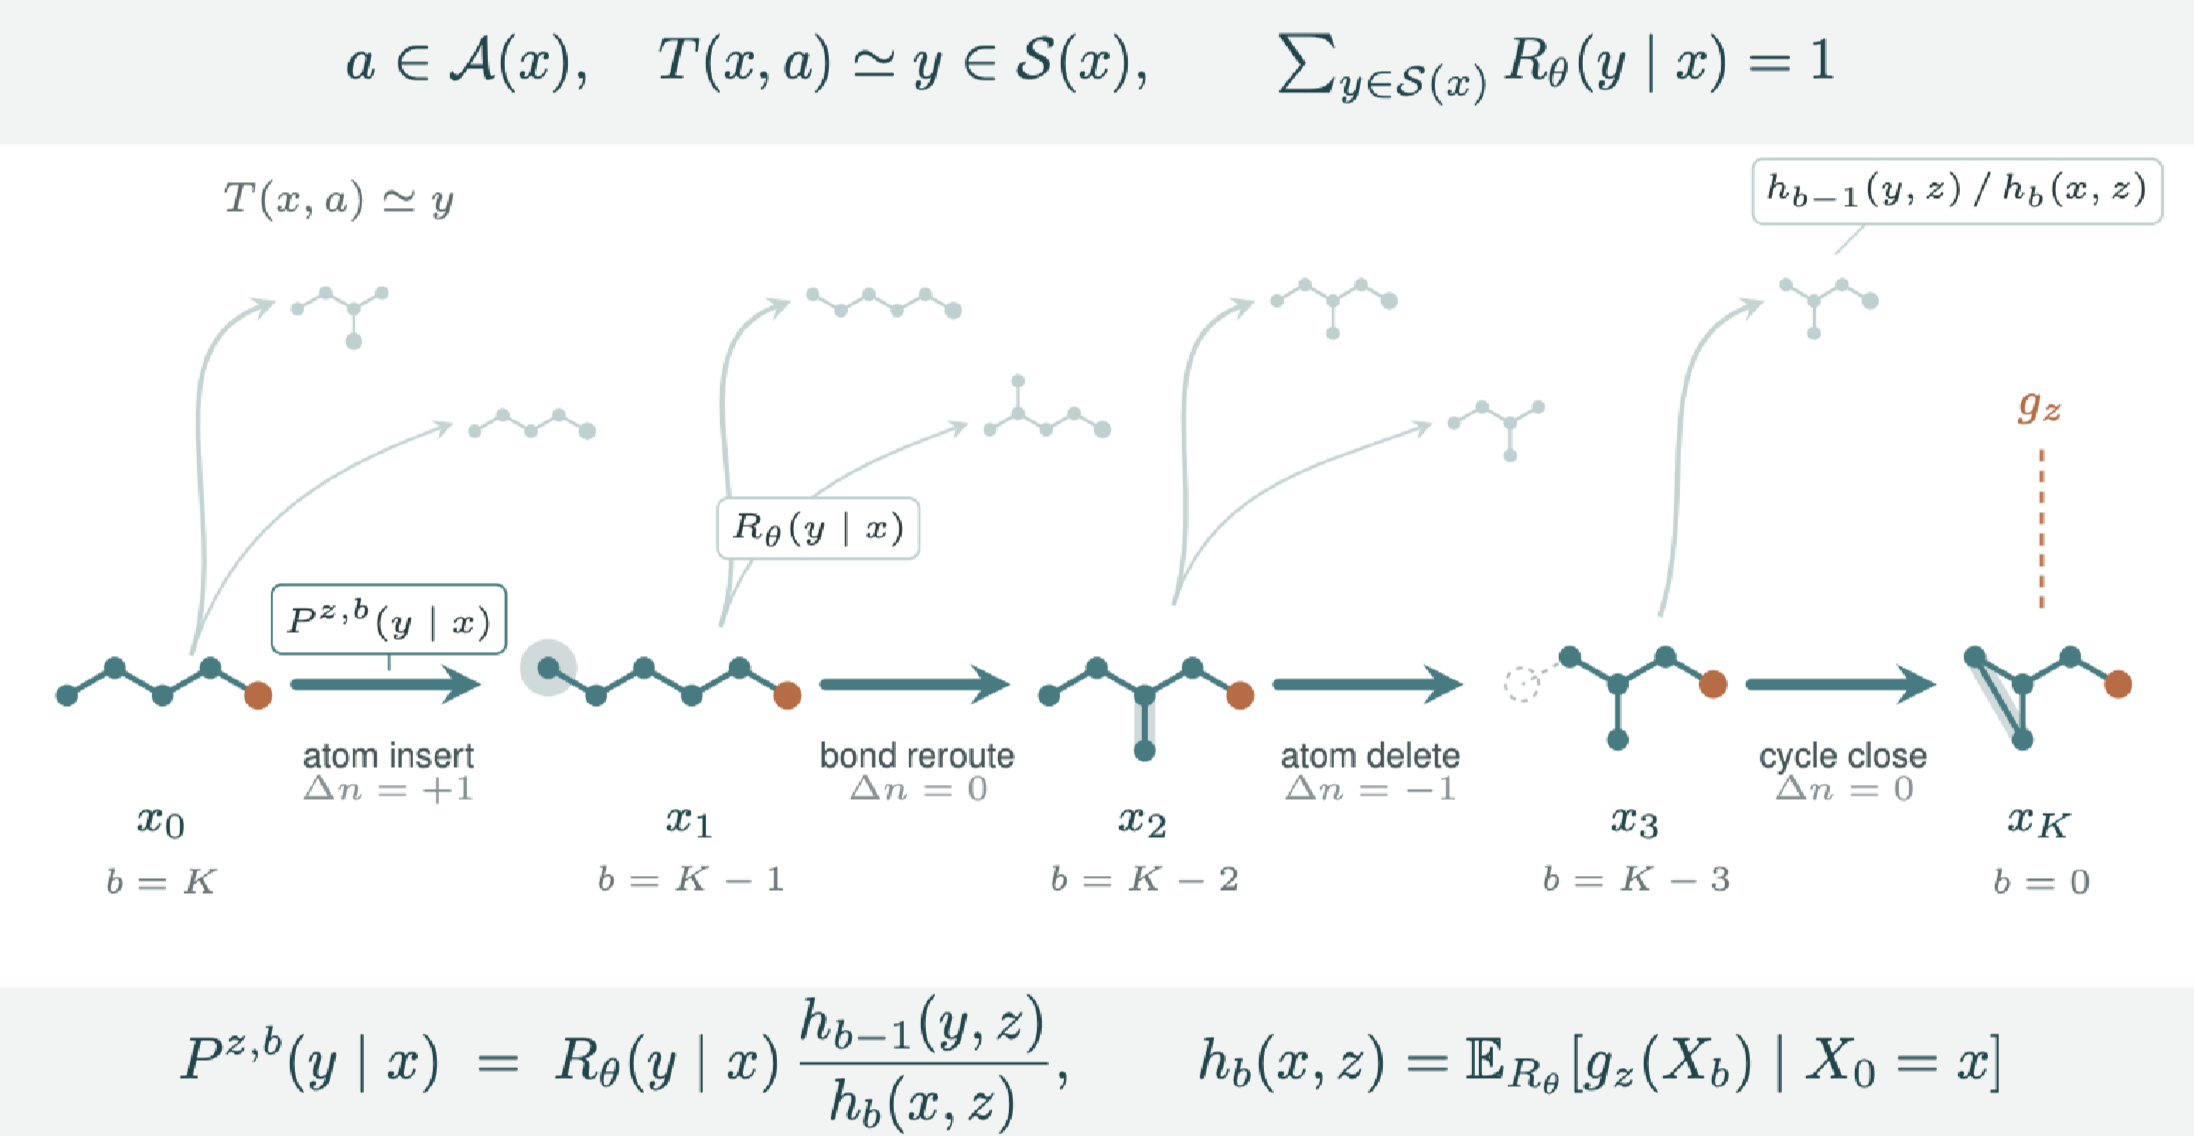
\includegraphics[width=\textwidth]{figures/fig1_overview.png}
\caption{\small Overview of COMPOSE. From a molecule \(x\), the graph-rewrite
executor admits edit marks \(a\in\mathcal A(x)\), which induce distinct canonical
successors \(y\in\mathcal S(x)\). The goal-independent reference kernel
\(R_\theta(y\mid x)\) assigns probability over this executable successor set, and
iterating \(R_\theta\) defines a trans-dimensional process over complete molecules.
For objective \(z\) and \(b\) remaining edits, finite-horizon control reweights each
reference transition by its remaining future value,
\(P^{z,b}(y\mid x)=R_\theta(y\mid x)h_{b-1}(y,z)/h_b(x,z)\), with
\(h_b(x,z)=\mathbb E_{R_\theta}[g_z(X_b)\mid X_0=x]\). Control therefore changes
which executable molecular transitions are preferred without introducing
transitions outside the support of \(R_\theta\).}
\label{fig:ppp}
\end{figure}

% ============================================================================
% GEM SECTION 2 --- Method.
%
% REWRITTEN 2026-08-27 FROM TEXT SUPPLIED VERBATIM.  Transcribed as given; no
% sentence reworded, shortened or resequenced.  Page fitting is the author's
% call, not this file's.
%
% The change from the previous version is density, not length-for-its-own-sake:
% the earlier compression sent the LEARNING OBJECTIVE and the factorization of
% R_theta to the appendix, which left Section 3.1's NLL decomposition without
% the construction it decomposes.  Eqs. (2)-(4) are restored to the body for
% exactly that reason.
%
% Load-bearing objects kept in the body, in order:
%   A(x)            what is executable
%   p_theta(a|x)    what is learned at mark level
%   R_theta(y|x)    why probability lives on molecular outcomes
%   L_ref           what the model actually learns
%   h_b             what "future-aware" means
%   P^{z,b}         how purpose changes the frozen process
%   Proposition 2   what the exact construction guarantees
%
% Still deliberately OUT of the body: SMC mechanics, Monte Carlo target
% estimators, architecture, full operator tables, ring-builder implementation,
% frontier algorithms, cache/inference machinery, proof details.
%
% APPENDIX POINTERS BELOW ARE AS SUPPLIED (N, O, L, G, Q).  They are transcribed
% verbatim and do NOT yet correspond to \label{}s in gem_appendix.tex; wire them
% before submission.
% ============================================================================

\section{COMPOSE: an executable molecular process}
\label{sec:method}

COMPOSE represents molecular design as control of a learned stochastic process
over complete molecules (Figure~\ref{fig:ppp}). The construction separates
three roles. An exact rewrite executor determines which molecular transitions
are \textbf{possible}. A goal-independent reference model learns which
executable transitions are \textbf{plausible}. Task-specific control then
reweights this frozen process according to which molecular futures are
\textbf{purposeful} for the current objective.

\subsection{Executable molecular state space}
\label{sec:gem-support}

Let
\[
  \mathcal X=\bigcup_{n=1}^{n_{\max}}\mathcal X_n
\]
denote the molecular state space, where $\mathcal X_n$ contains connected
molecular graphs with $n$ heavy atoms, declared atom and bond attributes, and
valid valences. Every $x\in\mathcal X$ is therefore a complete molecule rather
than a masked, corrupted, or partially specified state.

Transitions are typed graph rewrites. An edit mark $a$ specifies a rewrite
family, molecular operands, and a typed payload, and $T(x,a)$ denotes the
resulting graph. From state $x$, the executor exposes
\begin{equation}
  \mathcal A(x)
  =
  \left\{
    a:\; a\text{ matches } x
    \;\text{and}\;
    T(x,a)\text{ passes all executor guards}
  \right\}.
  \label{eq:gem-editset}
\end{equation}
The guards enforce the declared atom and bond vocabularies, valence
constraints, connectivity, and molecular-size bounds before an edit is
committed. Inadmissible states therefore have zero transition support rather
than being discouraged by a learned penalty.

The rewrite language contains atom insertion and deletion together with atom-,
bond-, and ring-level transformations (Appendix~N). Insertion and deletion
connect $\mathcal X_n$ to $\mathcal X_{n+1}$ and $\mathcal X_{n-1}$, while the
remaining transformations restructure a molecule at fixed size. COMPOSE is
therefore trans-dimensional: trajectories can grow, shrink, and reorganize
molecular graphs within one state space.

\begin{proposition}[Executable-support closure]
\label{prop:gem-closure}
For every $x\in\mathcal X$ and $a\in\mathcal A(x)$,
\[
  T(x,a)\in\mathcal X .
\]
\end{proposition}

Hence any stochastic process supported on the executable edit sets
$\{\mathcal A(x)\}_{x\in\mathcal X}$ remains in the declared molecular state
space. The proof and full rewrite semantics are given in Appendix~O.

The executor determines which molecular changes are possible. It does not
determine how probability should be distributed among them.

\subsection{Learning a molecular reference process}
\label{sec:gem-reference}

We learn a goal-independent stochastic law over executable edits. Writing a
mark as $a=(k,o,\eta)$, with rewrite family $k$, operands $o$, and typed payload
$\eta$, the reference model factorizes
\begin{equation}
  p_\theta(a\mid x)
  =
  p_\theta(k\mid x)\,
  p_\theta(o,\eta\mid k,x),
  \qquad a\in\mathcal A(x).
  \label{eq:gem-factorization}
\end{equation}
Normalization is restricted to candidates admitted by the executor. The model
receives no design objective, remaining budget, or downstream task information.
Thus $p_\theta$ models molecular transition structure independently of the
purpose for which the process will later be controlled.

The stochastic object used for control is a distribution over \textbf{molecular
successors}, not raw edit marks. Different marks can produce the same molecule
because of graph symmetries, equivalent matches, or alternative internal rewrite
descriptions. For a canonical successor $y$, define its executable fiber
\[
  \mathcal G_y(x)
  =
  \{a\in\mathcal A(x): T(x,a)\simeq y\},
\]
where $\simeq$ denotes registered molecular canonicalization. Let $\mathcal
S(x)$ denote the distinct non-self canonical successors of $x$. We define
\begin{equation}
  R_\theta(y\mid x)
  =
  \frac{
    \sum_{a\in\mathcal G_y(x)} p_\theta(a\mid x)
  }{
    \sum_{y'\in\mathcal S(x)}
    \sum_{a\in\mathcal G_{y'}(x)} p_\theta(a\mid x)
  },
  \qquad y\in\mathcal S(x).
  \label{eq:gem-rtheta}
\end{equation}
This quotient is important. A molecular transition does not become more probable
merely because symmetry gives the executor several syntactic ways to describe
it. State-level control therefore acts only after canonicalization.

We train $R_\theta$ from executable teacher transitions. If $y_i^\star$ is the
realized canonical successor of state $x_i$, the reference objective is
\begin{equation}
  \mathcal L_{\mathrm{ref}}(\theta)
  =
  -\frac{1}{N}\sum_{i=1}^{N}\log R_\theta(y_i^\star\mid x_i).
  \label{eq:gem-refloss}
\end{equation}
Every teacher transition is replayed through the same executor used at
inference. Targets and compiled programs are used to construct supervision but
are not supplied to the reference model at inference. We learn this reference
process once and keep it fixed across downstream objectives.

Equations~\eqref{eq:gem-factorization}--\eqref{eq:gem-refloss} also motivate the
decomposition in Section~\ref{sec:gem-exp-rtheta}: the family head learns
\textbf{which kind of edit} is appropriate, while the within-family law learns
\textbf{which molecular successor} is appropriate for the current state.

\subsection{Finite-horizon control of the frozen process}
\label{sec:gem-control}

Task information enters only after the molecular reference process has been
learned. Let $z$ denote a design objective and $g_z:\mathcal X\rightarrow
\mathbb R_{\geq0}$ its terminal desirability. For $b$ remaining molecular
transitions, define
\begin{equation}
  h_0(x,z)=g_z(x),
  \qquad
  h_b(x,z)
  =
  \sum_{y\in\mathcal S(x)} R_\theta(y\mid x)\, h_{b-1}(y,z).
  \label{eq:gem-backward}
\end{equation}
Equivalently,
\[
  h_b(x,z)
  =
  \mathbb E_{R_\theta}\!\left[ g_z(X_b)\mid X_0=x \right].
\]
This distinction is central. A property model scores \textbf{the molecule
currently in hand}. The backward value $h_b$ instead scores \textbf{what remains
reachable from that molecule within the remaining budget}.

For $h_b(x,z)>0$, the finite-horizon Doob transform defines
\begin{equation}
  P^{z,b}(y\mid x)
  =
  R_\theta(y\mid x)\,
  \frac{h_{b-1}(y,z)}{h_b(x,z)} .
  \label{eq:gem-central}
\end{equation}
The controller therefore changes probability only among molecular transitions
already supported by the frozen reference process.

\begin{proposition}[Finite-horizon molecular control]
\label{prop:gem-doob}
Starting from $x_0$ with budget $K$, applying
Equation~\eqref{eq:gem-central} at each step yields
\[
  \Pr\nolimits_{P^z}(X_K=y\mid X_0=x_0)
  =
  \Pr\nolimits_{R_\theta}(X_K=y\mid X_0=x_0)\,
  \frac{g_z(y)}{h_K(x_0,z)} .
\]
\end{proposition}

Thus exact backward values realize the $g_z$-tilted terminal law while
introducing no transition outside the executable reference support. The proof
and precise terminal-state assumptions are given in Appendix~O.

Exact backward computation requires enumerating the reachable molecular state
graph and is infeasible at molecular scale. We therefore learn a goal- and
budget-conditioned approximation
\begin{equation}
  h_\phi(x,z,b)\approx
  \mathbb E_{R_\theta}\left[ g_z(X_b)\mid X_0=x \right]
  \label{eq:gem-hphi}
\end{equation}
from finite-budget continuations of the frozen reference process. Replacing $h$
by $h_\phi$ in Equation~\eqref{eq:gem-central} gives the scalable future-value
controller. Approximation error may change which legal successor is preferred,
but it cannot introduce transitions outside the support of $R_\theta$. We
therefore reserve the exact terminal-reweighting guarantee for the exact
$h$-transform. Future-value supervision and sampling algorithms are given in
Appendices~G and~Q.

Because control is recomputed from the molecule actually reached, the same
process also supports intervention after execution begins. If an objective
changes from $z$ to $z'$ after reaching $x_\tau$, control simply resumes from
$x_\tau$ under $z'$; no parameter of $R_\theta$ changes.
Section~\ref{sec:gem-exp-lookahead} tests whether retaining this realized
molecular progress is useful in practice.

\paragraph{Executable transformations at longer time scales.}
\label{sec:gem-macros}
Some useful molecular changes require several primitive rewrites before their
value becomes visible. For molecular optimization, COMPOSE therefore exposes a
small set of temporally extended transformations, including linked and fused
ring construction and ring-local refinement. These operations introduce no
additional molecular support: they compile into the same primitive executable
rewrites, and every committed intermediate is checked by the same executor. The
controller chooses the transformation semantics, while the frozen reference law
ranks its legal molecular realizations. Full construction, refinement, and
qualification details are given in Appendix~L.

% ============================================================================
% GEM SECTION 3 --- Experiments.
%
% REWRITTEN 2026-08-27 FROM TEXT SUPPLIED VERBATIM.  The prose below is
% transcribed as given; no sentence has been reworded, shortened or resequenced
% to fit the page limit.  Page fitting is the author's call, not this file's.
%
% The organising change from the previous version is that 3.2 now states the
% GuacaMol -> frozen R_theta -> ZINC transfer explicitly, as a property of the
% reference process rather than as an OOD-generalisation claim.
%
% TWO PLACEHOLDERS REMAIN, exactly as supplied.  They are NOT results:
%   [Insert matched 800-source result here.]
%   [Insert final frozen 30-cell x 3-run results here.]
% Table 1 carries the matching bracketed cells.  Nothing here may be presented
% as measured until those are filled from a checked artifact.
% ============================================================================

\section{Experiments}
\label{sec:gem-experiments}

Our experiments address three questions. First, we ask whether the frozen reference
law learns state-dependent preferences among executable molecular edits. Second,
we test whether a reference process learned once on GuacaMol transfers unchanged
to externally defined molecular-design benchmarks. Finally, we study
trajectory-level capabilities that endpoint benchmarks do not capture: using
downstream reachability to guide molecular edits, retargeting realized molecular
states when objectives change, and enforcing constraints throughout a
trajectory.

\subsection{The reference process learns state-dependent edit preferences}
\label{sec:gem-exp-rtheta}

The rewrite system specifies which molecular edits are executable from a given
state, but it does not determine how probability should be distributed among
them. We therefore test whether the frozen reference law $R_\theta$ learns
state-dependent transition preferences beyond the global frequencies of
different edit families.

We evaluate 3{,}545 held-out transitions whose source molecules are disjoint
from reference-law training. As a matched baseline, we assign probability
according to empirical edit-family frequencies from the training set while
preserving the same executable support and canonical successor set as
$R_\theta$. The comparison therefore isolates how probability is allocated among
the molecular transitions available from each state.

$R_\theta$ reduces canonical-successor NLL from 5.37 to 3.90 nats relative to
this empirical-family baseline. A matched decomposition shows that 86.7\% of the
improvement comes from learning which successor is appropriate for the current
molecule, rather than simply learning which edit families are common overall
(\cref{tab:rtheta-cells}). The learned signal is therefore primarily state
specific: the executor supplies the available molecular transitions, while
$R_\theta$ learns how preference should be distributed across them.

We keep $R_\theta$ fixed in all subsequent experiments and use it as a
goal-independent reference process for molecular design. Its transition
probabilities are not intended to represent physical kinetics or synthetic-route
likelihoods. Results restricted to edit families with data-backed transition
supervision are reported in \cref{app:exp-rtheta}.

\subsection{A molecular process learned once transfers to external design tasks}
\label{sec:gem-exp-external}

We next evaluate whether the molecular process learned on GuacaMol can be reused
without retraining $R_\theta$. We keep the reference process and executable
rewrite system fixed and apply COMPOSE to two external benchmarks with different
design objectives: similarity-constrained QED editing on ZINC-250k, where
molecules can grow or shrink during editing, and protein-specific lead
optimization, where molecular properties define feasibility and docking score
provides the optimization objective. Only the task-specific controller changes
between these settings.

\paragraph{Similarity-constrained QED editing.}
We first consider the ZINC-250k editing benchmark used by GrIDDD
\citep{ninniri2025griddd}. Source molecules have QED in $[0.7,0.8]$, and a source
is counted as solved if at least one of $K$ returned molecules reaches QED
$\geq 0.9$ while maintaining Morgan-fingerprint Tanimoto similarity $\geq 0.4$ to
the source. GrIDDD is a particularly relevant comparator because its generative
process can insert and delete nodes, allowing molecular size to change during
editing. Its reported model is trained directly on ZINC-250k.

For COMPOSE, the GuacaMol-trained $R_\theta$ from \cref{sec:gem-exp-rtheta} is
left unchanged. A QED-specific controller is fit on development sources disjoint
from evaluation and acts on the same executable molecular process. Each of the
$K$ returned candidates corresponds to one controlled trajectory. We count a
trajectory as successful when it first reaches the target region, and do not
retrospectively add intermediate molecules to the candidate set.

On the official 800-source panel, COMPOSE solves 446 of the 800 sources
(55.8\%, 95\% CI $[52.3,59.2]$) with $K=8$, compared with the 45.1\% success
reported by GrIDDD with $K=20$ (\cref{tab:external}). COMPOSE therefore solves
more sources while returning fewer than half as many candidate trajectories per
source. Among solved sources with at least two distinct non-source candidates,
the mean within-source pairwise Tanimoto distance is 0.4999.

\paragraph{Similarity-constrained lead optimization.}
We next evaluate the same frozen reference process on the GenMol T4 benchmark
\citep{lee2025genmol}, which combines molecular feasibility with a
protein-specific optimization objective. The benchmark contains five protein
targets, three seed molecules per target, and similarity thresholds
$\delta\in\{0.4,0.6\}$. Returned molecules must satisfy QED $\geq 0.6$, SA
$\leq 4$, and Morgan-fingerprint Tanimoto similarity $\geq\delta$ to the seed.
Among molecules satisfying these constraints, performance is measured by
QuickVina2 docking score, with lower scores indicating stronger predicted
binding.

We retain the same GuacaMol-trained $R_\theta$ and executable rewrite system used
above, replacing only the task-specific controller. Here QED, SA, and similarity
determine whether a candidate is eligible, while docking provides the
optimization signal. Because these feasibility checks are inexpensive, they are
evaluated before the protein oracle and docking calls are reserved for eligible
molecules.

\begin{table}[!ht]
\centering\footnotesize\setlength{\tabcolsep}{4pt}
{\renewcommand{\arraystretch}{1.25}%
\begin{tabular}{ll >{\columncolor{composeteal!15}}r rrr >{\columncolor{composeteal!15}}r rrr}
\toprule
& Seed & \multicolumn{4}{c}{$\delta=0.4$} & \multicolumn{4}{c}{$\delta=0.6$} \\
\cmidrule(lr){3-6}\cmidrule(lr){7-10}
Target & score & \textbf{COMPOSE} & GenMol & RetMol & GraphGA & \textbf{COMPOSE} & GenMol & RetMol & GraphGA \\
\midrule
PARP1 & -7.3 & \textbf{-10.7} & -10.6 & -9.0 & -8.3 & \textbf{-11.1} & -10.4 & --- & -8.6 \\
 & -7.8 & \textbf{-11.5} & -11.0 & -10.7 & -8.9 & \textbf{-10.9} & -9.7 & --- & -8.1 \\
 & -8.2 & \textbf{-11.6} & -11.3 & -10.9 & --- & \textbf{-10.2} & -9.2 & --- & --- \\
FA7 & -6.4 & \textbf{-10.2} & -8.4 & -8.0 & -7.8 & \textbf{-8.7} & -7.3 & -7.6 & -7.6 \\
 & -6.7 & \textbf{-8.9} & -8.4 & --- & -8.2 & -7.2 & \textbf{-7.6} & --- & \textbf{-7.6} \\
 & -8.5 & \textbf{-9.3} & --- & --- & --- & \textbf{-7.9} & --- & --- & --- \\
5HT1B & -4.5 & -11.7 & \textbf{-12.9} & -12.1 & -11.7 & \textbf{-13.4} & -12.1 & --- & -11.3 \\
 & -7.6 & -11.2 & \textbf{-12.3} & -9.0 & -12.1 & -11.1 & \textbf{-12.0} & -10.0 & \textbf{-12.0} \\
 & -9.8 & -11.4 & \textbf{-11.6} & --- & --- & --- & \textbf{-10.5} & --- & --- \\
BRAF & -9.3 & --- & \textbf{-10.8} & --- & -9.8 & --- & --- & --- & --- \\
 & -9.4 & -11.2 & -10.8 & \textbf{-11.6} & --- & \textbf{-10.6} & -9.7 & --- & --- \\
 & -9.8 & -10.9 & -10.6 & --- & \textbf{-11.6} & --- & \textbf{-10.5} & --- & -10.4 \\
JAK2 & -7.7 & \textbf{-10.3} & -10.2 & -8.2 & -8.7 & \textbf{-9.3} & \textbf{-9.3} & --- & -8.1 \\
 & -8.0 & -9.8 & \textbf{-10.0} & -9.0 & -9.2 & \textbf{-9.7} & -9.4 & --- & -9.2 \\
 & -8.6 & \textbf{-10.5} & -9.8 & --- & --- & \textbf{-10.2} & --- & --- & --- \\
\bottomrule
\end{tabular}}
\caption{\small\textbf{Similarity-constrained lead optimization (GenMol T4).} QuickVina2 docking score of the best feasible lead, lower is better, subject to QED $\geq0.6$, SA $\leq4$, and Tanimoto similarity $\geq\delta$ to the seed. Baseline values are from GenMol Table 4; bold marks the best entry in each cell. COMPOSE is feasible in 26/30 cells, matching GenMol, and improves the paired mean by $0.335$ kcal/mol over the 23 cells where both are feasible (95\% CI $0.019$--$0.651$), using 500 docking-oracle evaluations per cell against 3{,}000 for the published GenMol result.}
\label{tab:t4}
\end{table}


COMPOSE returns a feasible molecule in \TFourCoverage{} of the 30 benchmark
settings, matching GenMol's coverage (\cref{tab:t4}). Across the \TFourPairedN{}
settings where both methods return a feasible molecule, COMPOSE improves the
paired mean docking score by $0.335$ kcal/mol (95\% CI $0.019$--$0.651$ in favor
of COMPOSE). This performance is obtained with 500 docking-oracle evaluations per
setting, compared with 3{,}000 evaluations underlying the published GenMol
result, a sixfold reduction. Since many individual docking differences are
comparable to replicate variation, we use the paired aggregate as the primary
comparison rather than interpreting small cell-level differences separately.

\subsection{Capabilities beyond fixed-objective endpoint optimization}
\label{sec:gem-exp-capabilities}

Endpoint benchmarks score the molecule returned after optimization, but do not
capture how decisions are made or revised along the trajectory. Because every
COMPOSE state is a complete molecule, control can use downstream reachability,
resume from a realized intermediate after an objective change, or restrict which
molecular states may be visited.

\paragraph{Future reachability changes multi-step edit decisions.}
An edit that improves immediate similarity can still eliminate every successful
continuation within the remaining budget. We test this on 65 held-out
source--target pairs, each with a certified executable path to the target and
sources disjoint from development. The local and future-aware policies share the
same frozen $R_\theta$, target, edit budget, and executable successors. They
differ only in whether the next edit is selected by immediate target similarity
or by the continuations available over the remaining budget.
Local selection reaches 26 of 65 targets, whereas future-aware control reaches
40, rescuing 14 of the 39 local failures without losing a local success
(\cref{tab:mechanism}). In one deterministic rescue, the locally preferred edit
has higher immediate similarity but removes the successful continuation, while a
slightly less similar edit preserves a path to the target. Exhaustive lookahead
is not required: using $h_\phi$ to prioritize a single successor preserves the
40/65 recovery rate while evaluating 34.6\% of the continuations required by
all-candidate lookahead. The full prioritization comparison is reported in
\cref{app:exp-lookahead}.

\paragraph{Realized molecular states can be retargeted after an objective change.}
Starting from $x_0$, we execute three edits under an initial objective and then
switch objectives at the realized state $x_3$. We compare continuing from $x_3$
with restarting from $x_0$, holding the new objective and remaining edit budget
fixed.
Across 40 held-out molecules, continuing from $x_3$ improves post-switch utility
in both directions: $0.302\,[0.186,0.413]$ for the potency-first objective and
$0.176\,[0.069,0.283]$ for the developability-first objective
(\cref{tab:mechanism}). The continued trajectories also move toward the new
objective rather than preserving the preference under which $x_3$ was reached.
Retargeting requires no update to $R_\theta$; control resumes from the realized
molecular state under the new objective.

\paragraph{Pathwise constraints act on the molecular trajectory.}
Some molecular requirements must hold at every intermediate rather than only for
the returned endpoint. COMPOSE enforces such statewise constraints by removing
violating successors before the reference kernel is normalized. We compare this
support restriction with endpoint-only filtering under matched sources,
objectives, and edit budgets.
On the developmental panel, 16 of 24 endpoint-feasible trajectories contained at
least one intermediate constraint violation, showing that endpoint feasibility
can hide inadmissible paths. Support-restricted control excludes such
intermediates by construction. We report the matched effect on optimization
performance and the full protocol in \cref{app:exp-pathwise}.



\begin{table}[!ht]
\centering\small\setlength{\tabcolsep}{7pt}
\begin{tabular}{@{}lrrr@{}}
\toprule
Method & Trajectories/source & Success $\uparrow$ & Diversity $\uparrow$ \\
\midrule
GrIDDD  & $20$ & $45.1\%$          & $0.283$ \\
COMPOSE & $8$  & $\mathbf{55.8\%}$ & $\mathbf{0.4999}$ \\
\bottomrule
\end{tabular}
\caption{\small\textbf{Similarity-constrained QED editing on ZINC-250k.} A source
is solved if at least one returned molecule reaches QED $\geq0.9$ while retaining
Morgan-fingerprint Tanimoto similarity $\geq0.4$ to the source. GrIDDD is trained
directly on ZINC-250k; COMPOSE transfers its GuacaMol-trained $R_\theta$ without
retraining, and solves more sources using fewer than half as many candidate
trajectories per source ($95\%$ CI $[52.3,59.2]$). Diversity is the mean
within-source pairwise Tanimoto distance over distinct non-source candidates,
averaged over solved sources returning at least two; GrIDDD does not fully
specify its diversity evaluator, so the two diversity entries are reported as
published rather than as an exactly matched comparison (\cref{app:bench-qed}).}
\label{tab:external}
\end{table}

\begin{table}[!ht]
\centering\small\setlength{\tabcolsep}{6pt}
\begin{tabular}{@{}p{0.21\textwidth} p{0.30\textwidth} p{0.41\textwidth}@{}}
\toprule
Trajectory-level capability & Matched comparison & Main finding \\
\midrule
Future-aware control & remaining-budget vs.\ local selection
  & \textbf{40/65} vs.\ 26/65 targets reached \\
\addlinespace[2pt]
Dynamic retargeting & continue from $x_3$ vs.\ restart from $x_0$
  & improves post-switch utility in both objective switches \\
\addlinespace[2pt]
Pathwise constraints & support restriction vs.\ endpoint-only filtering
  & endpoint-only filtering permits hidden intermediate violations; support
    restriction prevents them by construction \\
\bottomrule
\end{tabular}
\caption{\small\textbf{Trajectory-level capabilities of the frozen molecular
process.} Each comparison changes how the trajectory is controlled while keeping
the reference process $R_\theta$ fixed. Confidence intervals, prioritization
results, and full protocols are reported in \cref{app:experiments}.}
\label{tab:mechanism}%
\label{fig:mechanism}
\end{table}

% ============================================================================
% GEM SECTION 4 --- Discussion.  BOTH PARAGRAPHS ARE THE MAP'S TEXT VERBATIM.
% Nothing is added and nothing is trimmed here.  (An earlier revision of this
% file carried two extra sentences lifted from the full-paper discussion --
% the "not unique to COMPOSE" concession and the exact-backward-values
% qualification.  Those were not in the map and have been removed.  If they
% are wanted back, that is an authoring decision, not a fitting decision.)
% ============================================================================
\section{Discussion}
\label{sec:discussion}

COMPOSE is built around a reference process that is learned independently of any
downstream objective. In our experiments, the same GuacaMol-trained $R_\theta$ is
reused for variable-size editing on ZINC-250k and for protein-specific lead
optimization, with only the controller changing between tasks. Representing the
intermediate states explicitly as molecules also makes it possible to look ahead
before committing an edit, continue from a molecule already reached when the
objective changes, and restrict which molecular states can be visited along a
trajectory.

The current formulation still has important limits. Exact finite-horizon control
requires exact backward values, which are only tractable on small enumerable
state spaces. At molecular scale we instead rely on the learned approximation
$h_\phi$, so the exact terminal-law guarantee no longer applies. COMPOSE is also
limited by the rewrite vocabulary used to define its support. Chemistry that
cannot be expressed by those rewrites cannot be recovered through control.
Finally, the optimization experiments inherit the limitations of the property
models and docking scores used as objectives. Extending the rewrite process to
broader chemistry and testing it against experimentally measured objectives are
natural next steps.


\bibliography{references}
\bibliographystyle{plainnat}

\newpage
\appendix
% ============================================================================
% GEM APPENDIX.  GEM excludes the appendix from the 5-page limit, so every
% section removed from the body is carried here WHOLE AND UNCHANGED rather
% than summarized.  The files below are byte-identical copies of the
% paper_iclr2027 sources; do not edit them here.  Edit the full paper and
% re-copy, so the two versions cannot silently diverge.
% ============================================================================
\section*{Appendix}
\addcontentsline{toc}{section}{Appendix}

\section{Related work}
\label{app:related}
% ============================================================================
% RELATED WORK --- three paragraphs, each closing on the COMPOSE distinction.
%   P1  molecular generation/editing -> GrIDDD          -> our molecular process
%   P2  generator matching/Edit Flows -> MadSBM
%                                     -> Value Matching/pCoMole
%                                     -> our process/control decomposition
%   P3  InversionGNN/PepTune/AReUReDi/Routing by Reaching
%                                     -> our closed-loop multi-objective control
% No fourth "stochastic control" paragraph: Doob / Feynman-Kac / Schrodinger
% citations live in the preliminaries and Section 5.  Graph-GRPO is deliberately
% held for the extended related work unless we compare against it directly.
% ============================================================================
\label{sec:related}

Molecular generation spans latent-variable, graph-to-graph, reinforcement-learning, diffusion, and flow-based approaches, while molecular optimization has also been formulated directly through graph edits, fragment proposals, evolutionary operators, and MCMC transitions \citep{gomezbombarelli2018chemvae,jin2018jtvae,jin2019vjtnn,zhou2019moldqn,jensen2019graphga,xie2021mars,fu2021mimosa,vignac2023digress,campbell2024multiflow}. Recent work has begun to relax the fixed-size assumption of graph generation: GrIDDD introduces node insertion and deletion into discrete graph diffusion, allowing molecular graphs to grow and shrink during denoising \citep{ninniri2025griddd}. \method{} instead learns a goal-independent stochastic law over an explicit, state-dependent molecular rewrite space, making the transition process itself the object of subsequent control.

A related line of work treats generation and adaptation directly through stochastic processes. Generator matching provides a general framework for learning Markov generators from tractable conditional processes, while Edit Flows develops insertion, deletion, and substitution dynamics for variable-length discrete generation \citep{holderrieth2025generator,havasi2025editflows}. MadSBM is a close mathematical relative, formulating peptide generation as a controlled Markov process on an amino-acid edit graph, although its learned control constructs the generative transport rather than adapting an already learned molecular process \citep{goel2026madsbm}. Value Matching steers a frozen flow model through a learned value function, and pCoMole studies Pareto-constrained molecular editing with discrete flows \citep{jensen2026valuematching,pcomole2026}. Future-aware generative control is therefore not unique to \method{}: value-guided flow adaptation and pCoMole likewise use learned or rollout-estimated future value. Our distinction is the substrate on which that control operates. It is a learned canonical transition law over executable molecular graphs, which is what allows realized molecular states to be reused, retargeted, and constrained.

Multi-objective molecular design has been addressed through surrogate-based optimization, evolutionary search, and inference-time guidance of generative models. InversionGNN combines multi-property prediction with gradient-based Pareto search in discrete molecular space \citep{niu2025inversiongnn}, while PepTune and AReUReDi use discrete generative models with multi-objective tree search or Pareto-oriented refinement \citep{tang2025peptune,chen2025areuredi}. Routing by Reaching similarly composes pretrained GFlowNets for multi-objective generation at inference time \citep{yoon2026routing}. \method{} instead places multi-objective control on a reusable molecular transition process, so that future reachability and already-reached molecular states can participate directly in Pareto exploration.


\section{Preliminaries}
\label{app:preliminaries}
% ============================================================================
% PRELIMINARIES --- background only.  Nothing here is a contribution.
%
% Two subsections, deliberately.  The only external mathematics a reader needs
% before COMPOSE is a discrete-step Markov chain and the finite-horizon Doob
% h-transform.
%
% Deliberately excluded, because each is COMPOSE rather than background:
%   the executable rewrite space A(x); the trans-dimensional molecular state
%   space; canonical molecular successors; the reference-law training objective;
%   the h_phi amortization; and Pareto machinery.
%
% Generator matching was removed as a preliminary on 2026-08-20.  Giving it a
% subsection told the reader it is the training framework, which the shipped
% objective is not: R_theta is fitted by the productive canonical-successor
% identity likelihood and the exit rate is never optimized.  The exact relation
% to the corresponding block of Poisson generator matching is stated in Sec. 4.2
% AFTER the actual objective is defined, which is where it informs rather than
% misleads.  Do not reinstate it here.
%
% NOTE, notation: 3.2 indexes value by forward step (h_K = g, h_k = P_k h_{k+1})
% while Sec. 4.4 uses remaining budget (h_0 = g, h_b = R_theta h_{b-1}).  The
% paper emphasises remaining budget throughout, so both should be unified on the
% remaining-budget convention in the same pass that revises 4.4.  Left
% inconsistent here deliberately rather than creating a second mismatch.
% ============================================================================
\label{sec:prelim}

\subsection{Markov chains}
\label{sec:prelim-chain}

Let $\X$ be a discrete state space and $P_0,\dots,P_{K-1}$ a sequence of transition kernels defining a possibly time-inhomogeneous Markov chain over $K$ steps. Starting from $X_0=x_0$, the probability of a trajectory $x_{1:K}$ is
\begin{equation}
P(X_{1:K}=x_{1:K}\mid X_0=x_0)=\prod_{k=0}^{K-1}P_k(x_{k+1}\mid x_k).
\label{eq:chain}
\end{equation}
Thus each transition depends only on the current state and the step of the process, while the sequence of kernels determines a distribution over complete trajectories. In \method{}, fixed-budget molecular editing takes this form: each state is a complete molecular graph and each committed transition corresponds to one molecular edit.

\subsection{Finite-horizon Doob control}
\label{sec:prelim-ctrl}

We also recall finite-horizon control of a reference Markov chain. Let $g_z(x)\ge 0$ assign terminal desirability under goal $z$. Defining the backward value $h_K(x,z)=g_z(x)$ and
\begin{equation}
h_k(x,z)=\sum_{y} P_k(y\mid x)\,h_{k+1}(y,z),
\qquad
P^z_k(y\mid x)=P_k(y\mid x)\,\frac{h_{k+1}(y,z)}{h_k(x,z)},
\label{eq:doobprelim}
\end{equation}
gives the finite-horizon Doob $h$-transform wherever $h_k(x,z)>0$. Writing $P^z$ for the law of the chain run under these controlled kernels, the resulting terminal distribution is
\begin{equation}
P^{z}(X_K=y\mid X_0=x_0)
=\frac{P(X_K=y\mid X_0=x_0)\,g_z(y)}{\E_P\!\left[g_z(X_K)\mid X_0=x_0\right]}.
\label{eq:terminaltilt}
\end{equation}
The transform therefore reweights only transitions already present in the reference chain and introduces no new support. With exact backward values, it realizes the reference terminal distribution tilted by $g_z$. In \method{}, this construction provides the control law for molecular editing, with an amortized future-value model replacing exact backward computation in large molecular spaces.

\method{} instantiates these generative and control primitives on a state-dependent, trans-dimensional molecular rewrite space.


\section{The executable molecular process in full}
\label{app:process}
% ============================================================================
% SECTION 4 --- Methods
%   2.1 exact transition support (state space, A(x), executor, closure,
%       trans-dimensionality; ONE proposition; families -> app:operators)
%   2.2 learning which legal edits are plausible (generator matching; arrive
%       quickly at R_theta over canonical successors; source independence)
%   2.3 canonical molecular successors (worked example; why aggregation)
% Terminology contract: "connected, valence-admissible within the declared
% molecular state space", "reference edit law", "canonical molecular
% successor".  "exact" is used only of the executor's support and of canonical
% normalization.  No number appears in this section.
% COMPRESSED TO THE 9-PAGE LIMIT.  Detail relocated to app:operators and
% app:quotient, which are unlimited; do not re-expand here without cutting
% elsewhere.
% ============================================================================
\label{sec:process}

We develop \method{} as a reusable stochastic process over molecular edits and a finite-horizon controller over that process. \method{} realizes generative stochastic rewriting by repeatedly applying executable molecular edits under a learned, goal-independent transition law. An exact rewrite system first determines which transitions between complete molecular graphs are executable. We then learn a goal-independent reference law over this state-dependent support and push it forward to a canonical molecular successor kernel $R_\theta$. Finally, we control the frozen successor process through a budget-conditioned $h$-transform, using a learned future-value model $h_\phi$ to approximate the required backward values at molecular scale.

\subsection{Executable molecular transitions}
\label{sec:support}

\method{} represents every generative state as a complete molecular graph. Let $n_{\max}$ denote the maximum number of heavy atoms admitted by the declared molecular state space. For $n\in\{1,\dots,n_{\max}\}$, let $\X_n$ be the set of connected molecular graphs with $n$ heavy atoms whose node and edge attributes lie in the declared vocabularies of elements, bond orders, formal charges, and implicit hydrogens, and in which every atom satisfies its declared valence constraints. The molecular state space is
\begin{equation}
\X=\bigsqcup_{n=1}^{n_{\max}}\X_n.
\label{eq:statespace}
\end{equation}
Thus each state $x\in\X$ is a complete molecule rather than a masked, corrupted, or partially specified representation.

Molecular transitions are generated by typed graph rewrites. An edit mark $a$ specifies a rewrite type together with its molecular match and typed payload, and $\T(x,a)$ denotes the graph obtained by applying that rewrite to $x$. The full atom-, bond-, and ring-level edit language is specified in \cref{app:operators}. From a state $x$, the executor exposes only the finite, state-dependent set
\begin{equation}
\A(x)=\bigl\{\,a:\ a\ \text{matches}\ x\ \ \text{and}\ \ \T(x,a)\ \text{passes all executor guards}\,\bigr\}.
\label{eq:editset}
\end{equation}
Execution follows a propose--validate--commit rule: a successor is admitted only if its attributes remain in the declared vocabularies, affected valences are satisfied, the graph remains connected, and its heavy-atom count lies in $\{1,\dots,n_{\max}\}$. An edit that fails any guard contributes no transition to $\A(x)$. Inadmissible molecular states are therefore absent from the stochastic support rather than discouraged through a learned penalty.

The decomposition of $\X$ by heavy-atom count makes the process trans-dimensional. Each admitted edit changes heavy-atom count by at most one, yielding \emph{birth}, \emph{death}, or \emph{same-cardinality} transitions between $\X_n$ and $\X_{n+1}$, $\X_{n-1}$, or $\X_n$, respectively. Birth and death edits create or remove typed graph entities that participate in valence, connectivity, and ring perception rather than merely activating or deactivating padded coordinates. A trajectory may therefore grow, shrink, and restructure a molecular graph within a common state space.


Because membership in $\A(x)$ already encodes the guards defining $\X$, we have $\T(x,a)\in\X$ for every $x\in\X$ and $a\in\A(x)$\label{prop:closure}. Consequently every state reached by a stochastic process supported on $\{\A(x)\}_{x\in\X}$ remains in the declared molecular state space; the argument is given in \cref{app:theory}.

The legal edit sets $\A(x)$ therefore determine which molecular transitions are possible, but not how probability should be distributed among them. We next learn a goal-independent stochastic law over this executable support.

\subsection{Learned molecular reference process}
\label{sec:rtheta}

Having defined which molecular rewrites are executable, we next learn how probability is distributed over them. For every state $x$ with $\A(x)\neq\emptyset$, the reference model defines a normalized conditional law over legal edit marks,
\begin{equation}
p_\theta(a\mid x,t),\qquad\sum_{a\in\A(x)}p_\theta(a\mid x,t)=1,
\label{eq:marklaw}
\end{equation}
where $t$ is a progress variable. Writing an edit as $a=(k,o,\eta)$, with family $k$, matched molecular operands $o$, and typed payload $\eta$, we parameterize
\begin{equation}
p_\theta(a\mid x,t)=p_\theta(k\mid x,t)\,p_\theta(o,\eta\mid k,x,t).
\label{eq:hierarchical}
\end{equation}
A shared molecular encoder represents the current graph, while family-specific scorers normalize only over candidates admitted by the executor. The reference model receives no downstream objective, remaining budget, or task-specific constraint, and the original source molecule is not supplied as an additional conditioning variable. The source determines the initial state; task information enters later through support restrictions and control. Thus the learned reference law represents molecular \emph{plausibility} independently of molecular \emph{purpose}.

Supervision is obtained by compiling molecular endpoint pairs into executable edit programs. Every stored teacher transition is replayed through the same executor used at inference, so the model is trained only on transitions available to the deployed process. The compiler may use both endpoints to construct an edit program, but neither the target endpoint nor the program is available to the reference model at inference. Because multiple legal marks can execute to the same molecular graph, the learning objective is defined on the resulting molecular successor rather than on a particular syntactic realization. Let $R_{\theta,t}(y\mid x)$ denote the induced law over distinct committed molecular successors, formalized in \cref{sec:canonical}. For productive teacher transitions $x_i\rightarrow y^{\star}_i$, we minimize
\begin{equation}
\mathcal{L}_{\mathrm{ref}}(\theta)=-\frac{\sum_i w_i\log R_{\theta,t_i}(y^{\star}_i\mid x_i)}{\sum_i w_i},
\label{eq:refloss}
\end{equation}
where $w_i$ is the registered weight under the declared editing measure. Terminal rows do not enter this objective. \Cref{eq:refloss} therefore learns which committed molecular successor follows a state under that measure; it does not calibrate continuous-time holding rates.

This objective is related to generator matching but is not the generator-matching population objective. Writing the productive rate as $Q^{+}(y\mid x,t)=\Lambda(x,t)P(y\mid x,t)$, the corresponding generator-matching divergence separates pointwise into a productive-hazard term and a conditional-successor term proportional to $\Lambda^{\star}\KL(P^{\star}\,\|\,R_\theta)$. \method{} optimizes the successor component only: the hazard term is not optimized, and \cref{eq:refloss} is averaged under the declared family-weighted editing measure rather than the state--time marginal of the conditional-process mixture \citep{holderrieth2025generator}. \Cref{app:gm} gives the full decomposition and the precise measure-level distinction.

The learned mark law is not yet the molecular kernel used for control: distinct executable marks can yield the same molecular state. We therefore next push $p_\theta$ through the executor and aggregate probability by canonical molecular outcome.

\subsection{Canonical molecular successors}
\label{sec:canonical}

We now push the learned edit law through the executor to obtain a stochastic process over distinct molecular states. Multiple legal marks can produce the same molecular graph because of graph symmetries, equivalent matches, or alternative internal rewrite descriptions. For a canonical successor $y$, define its successor fiber
\begin{equation}
\Gset_y(x)=\bigl\{\,a\in\A(x):\ \T(x,a)\simeq y\,\bigr\},
\label{eq:sucfiber}
\end{equation}
where $\simeq$ denotes equivalence under the registered molecular canonicalization. The induced probability of $y$ is
\begin{equation}
\bar p_{\theta,t}(y\mid x)=\sum_{a\in\Gset_y(x)}p_\theta(a\mid x,t).
\label{eq:pushforward}
\end{equation}
Thus probability assigned to a molecular transition is the aggregate mass of every executable mark that realizes it. For example, deleting any of the three symmetry-equivalent terminal methyl carbons in 2-methylpropane, $\op{CC(C)C}$, produces propane; canonicalization exposes propane once with the combined probability of those marks rather than overweighting it because of representational multiplicity.

Fixed-budget editing counts committed changes of molecular state rather than internal mark draws. Let $\Sset(x)$ denote the distinct non-self canonical successors admitted by this convention. Conditioning the pushforward distribution on a committed state change defines the molecular reference kernel
\begin{equation}
R_{\theta,t}(y\mid x)=\frac{\one\{y\in\Sset(x)\}\,\bar p_{\theta,t}(y\mid x)}{\sum_{y'\in\Sset(x)}\bar p_{\theta,t}(y'\mid x)}.
\label{eq:rtheta}
\end{equation}
If $\Sset(x)=\emptyset$, $x$ is terminal for the committed molecular process. For $b>0$, such a state has $h_b(x,z)=0$ under the backward recursion of \cref{sec:control}; trajectories terminating before the declared horizon therefore carry zero mass in the exact-$K$-step controlled terminal law. Otherwise $R_{\theta,t}$ is a normalized law over distinct molecular successors, and iterating it defines the goal-independent reference process optimized by \cref{eq:refloss}. We suppress $t$ and write $R_\theta(y\mid x)$ when the registered progress convention is fixed; canonical self-events and other non-committed outcomes are detailed in \cref{app:quotient}.

\begin{proposition}[Canonical normalization]
\label{prop:canonical}
For every nonterminal state $x$, $\sum_{y\in\Sset(x)}R_{\theta,t}(y\mid x)=1$. Moreover, any refinement or coarsening of the internal mark representation that preserves the aggregate probability mass of every canonical successor fiber leaves $R_{\theta,t}$ unchanged. Consequently, state-level controllers that reweight $R_{\theta,t}$ using quantities defined on canonical molecular successors are invariant to such representational refinements.
\end{proposition}

This invariance relies on performing control after canonicalization: reweighting or truncating individual marks beforehand can reintroduce dependence on arbitrary edit multiplicities. With the goal-independent reference process now defined on complete molecular states, we next control this frozen kernel toward finite-horizon design objectives.


\section{Finite-horizon control in full}
\label{app:control}
% ============================================================================
% SECTIONS 4.4-4.8: control, folded into Section 4 (Method).
%   4.4 exact finite-horizon control (backward value, controlled kernel, theorem)
%   4.5 goal-conditioned value learning
%   4.6 immediate prediction vs future value
% "exact" appears here only of exact dynamic programming and of the exact
% terminal tilt UNDER AN EXACT h.  h_phi is amortized / learned / approximate
% and is never called exact.  No number appears in this section.
% ============================================================================
\subsection{Finite-horizon molecular control}
\label{sec:control}
\label{sec:doob}

Having defined the goal-independent molecular reference process $R_\theta$, we now introduce task-specific control without modifying that process. Let $z$ denote a design objective and $g_z:\X\rightarrow\R_{\ge0}$ its terminal desirability. For a remaining budget of $b$ molecular transitions, define the backward values
\begin{equation}
h_0(x,z)=g_z(x),\qquad
h_b(x,z)=\sum_{y\in\Sset(x)}R_\theta(y\mid x)\,h_{b-1}(y,z)
=\E_{R_\theta}\!\left[g_z(X_b)\mid X_0=x\right].
\label{eq:backward}
\end{equation}
Thus $h_b(x,z)$ evaluates a molecule by the desirability reachable from it after $b$ further transitions under the reference process. Unlike a score of the current molecule, it depends on the molecular futures that remain accessible through $R_\theta$.

For $h_b(x,z)>0$, the finite-horizon $h$-transform defines
\begin{equation}
R^{z,b}_\theta(y\mid x)=R_\theta(y\mid x)\,\frac{h_{b-1}(y,z)}{h_b(x,z)}.
\label{eq:doob}
\end{equation}
The controlled kernel therefore reweights the same canonical molecular successors according to their remaining future value: a transition may be preferred despite little immediate improvement if it preserves access to desirable states later in the trajectory. If $h_b(x,z)=0$, no state with positive terminal desirability is reachable within the remaining budget under the reference process, and we leave the controlled row undefined rather than introduce probability outside its support.

\begin{theorem}[Finite-horizon molecular control]
\label{thm:doob}
Let $R_\theta$ define the reference path measure over $K$ committed transitions from $x_0$, with trajectories terminating before $K$ assigned zero continuation mass, let $g_z$ be nonnegative and finite-valued, and suppose $0<h_K(x_0,z)<\infty$. Applying $R_\theta^{z,K-j}$ at step $j=0,\dots,K-1$ defines normalized controlled kernels whose support is contained in that of $R_\theta$, and whose terminal distribution satisfies
\begin{equation}
\Prob^{z}(X_K=y\mid X_0=x_0)=\Prob_{R_\theta}(X_K=y\mid X_0=x_0)\,\frac{g_z(y)}{h_K(x_0,z)}.
\label{eq:tilt}
\end{equation}
\end{theorem}

Thus exact backward values realize the $g_z$-tilted terminal law without introducing transitions outside the executable reference support. The proof is given in \cref{app:proofs}.

The guarantee is horizon-specific: before the terminal step, the controlled marginal is determined by the remaining backward value rather than directly by $g_z$, so early stopping does not in general realize the terminal tilt. Because every state of $R_\theta$ is a complete molecule and every transition an executable rewrite, $h_b(x,z)$ has a direct interpretation as future desirability from a realized molecular intermediate through its remaining executable continuations. Exact backward evaluation is tractable only when the relevant state graph can be enumerated. \Cref{sec:hphi} therefore replaces $h_b$ with a learned goal- and budget-conditioned approximation $h_\phi(x,z,b)$, retaining the same finite-horizon control interface at molecular scale.

\subsection{Learning goal- and budget-conditioned future value}
\label{sec:hphi}

Exact evaluation of the backward values in \cref{sec:control} requires propagating terminal desirability over the molecular states reachable within the remaining edit budget, which is infeasible in realistic molecular spaces. We therefore learn an amortized approximation $h_\phi$ while keeping the molecular reference process $R_\theta$ fixed. For objective $z$ and $b$ remaining transitions,
\begin{equation}
h_\phi(x,z,b)\approx h_b(x,z)=\E_{R_\theta}\!\left[g_z(X_b)\mid X_0=x\right].
\label{eq:hphi}
\end{equation}
The remaining budget is part of the prediction problem: the same molecule can have different future value under the same objective depending on how many executable transitions remain.

We construct supervision directly from the frozen reference process. From a molecular state $x$, $M$ independent $b$-step continuations give the Monte Carlo target
\begin{equation}
\widehat h_M(x,z,b)=\frac{1}{M}\sum_{m=1}^{M}g_z\!\left(X_b^{(m)}\right),
\qquad
X_b^{(m)}\sim R_\theta^{\,b}(\cdot\mid x).
\label{eq:mctarget}
\end{equation}
When $g_z$ is an indicator, this target estimates finite-budget reachability; for a general nonnegative desirability, it estimates expected future value. Training and validation are partitioned by molecular source so that states descended from the same source do not cross splits.

The exact backward values also satisfy the Bellman recursion in \cref{eq:backward}, which provides an additional source of supervision when adjacent-budget trajectory pairs are available. We use this consistency relation as an auxiliary training signal for the reachability-valued controller, while controllers trained on soft expected-desirability targets are fit directly to their Monte Carlo future-value estimates. In both cases, $h_\phi$ is trained to approximate the backward quantity defining the exact controller rather than an independent task-specific score. Architecture and training details for the respective future-value models are given in \cref{app:controller,app:mo-controller}.

This distinction is important when terminal desirability is derived from a learned property model $\widehat F_\psi$. The property model $\widehat F_\psi(x)$ estimates properties of the current molecule, whereas $h_\phi(x,z,b)$ estimates the desirability reachable from that molecule after $b$ further transitions of $R_\theta$. Property learning therefore estimates where value may lie; future-value learning propagates that value through the molecular process.

Replacing the exact backward value in \cref{eq:doob} yields the scalable controlled kernel
\begin{equation}
P_\phi(y\mid x,z,b)=\frac{R_\theta(y\mid x)\,h_\phi(y,z,b-1)}{\displaystyle\sum_{y'\in\Sset(x)}R_\theta(y'\mid x)\,h_\phi(y',z,b-1)},
\qquad y\in\Sset(x),
\label{eq:central}
\end{equation}
whenever the denominator is positive. If $h_\phi=h$, \cref{eq:central} recovers the exact finite-horizon transform of \cref{thm:doob}. With learned $h_\phi$, approximation error can change how probability is allocated among executable successors, but cannot introduce a transition outside the support of $R_\theta$. Exact terminal reweighting remains a guarantee of the exact $h$-transform and is not claimed for the learned approximation.

\subsection{Sampling the controlled molecular process}
\label{sec:sampling}

At inference, \method{} applies the controlled kernel in \cref{eq:central} recursively over realized molecular states. Given the current molecule $x$, objective $z$, and remaining budget $b$, the executor enumerates the canonical successor set $\Sset(x)$; $R_\theta$ assigns goal-independent reference probability to these successors, and $h_\phi$ reweights them by their predicted remaining future value. After sampling and committing a successor, the resulting molecule becomes the next state and the budget is decremented. Recomputing the controlled law after every committed edit therefore yields a closed-loop molecular trajectory whose decisions depend on the state actually reached rather than on a trajectory fixed in advance.

When $\Sset(x)$ can be evaluated directly, we sample from the normalized kernel in \cref{eq:central}. The same row can alternatively be sampled by rejection whenever $h_\phi$ admits a finite envelope: proposing from $R_\theta(\cdot\mid x)$ and accepting in proportion to $h_\phi$ recovers the controlled distribution conditional on acceptance. For objectives whose desirable futures carry little reference mass, direct sampling can allocate insufficient computation to useful trajectories. We instead use a Feynman--Kac sequential Monte Carlo construction. Particles propagate under the frozen reference process $R_\theta$, and a transition $x\to y$ with $b$ remaining steps receives incremental potential
\begin{equation}
G_b(x,y)=\frac{h_\phi(y,z,b-1)}{h_\phi(x,z,b)}.
\label{eq:fk}
\end{equation}
Particles are resampled when effective sample size falls below $N/2$. When $h_\phi$ equals the exact backward value, these potentials recover the finite-horizon Doob-controlled path law of \cref{sec:control}. With learned $h_\phi$, the same value approximation acts as a twisting function for the reference particle system; the resulting finite-particle procedure is an approximation whose target and boundary conditions are detailed in \cref{app:sampling}.

For objectives defined by a target region $\Bset_z$, we stop prospectively at the first realized hit,
\begin{equation}
\tau=\min\!\left(\{t\le K:X_t\in\Bset_z\}\cup\{K\}\right).
\label{eq:stop}
\end{equation}
A reached molecule is returned when the target region is entered; if no hit occurs, the trajectory continues to its declared budget. Intermediate states are not retrospectively collected as additional samples: one controlled trajectory produces one returned candidate. Objectives without a first-hit interpretation are sampled to the declared horizon.

\subsection{Preference-conditioned multi-objective control}
\label{sec:preferences}

The preceding construction applies to any nonnegative terminal desirability $g_z$. To control \method{} under competing molecular objectives, let $\widehat{\mathbf F}_\psi(x)=\bigl(\widehat F_{\psi,1}(x),\ldots,\widehat F_{\psi,m}(x)\bigr)\in[0,1]^m$ denote frozen property scores oriented so that larger values are preferred, and let $\lambda\in\Delta^{m-1}$ specify a preference over objectives. We define the weighted Chebyshev shortfall
\begin{equation}
L_\lambda(x)=\max_{i=1,\ldots,m}\ \lambda_i\bigl(1-\widehat F_{\psi,i}(x)\bigr).
\label{eq:cheby}
\end{equation}
Unlike an additive scalarization, the maximum is determined by the most limiting preference-weighted objective, preventing improvement in one property from arbitrarily compensating for poor performance on another.

We convert this shortfall into the nonnegative terminal desirability required by the finite-horizon controller,
\begin{equation}
g_\lambda(x)=\exp\!\left(-\frac{L_\lambda(x)}{\tau_\lambda}\right),
\qquad
\tau_\lambda=\operatorname{Std}_{x\sim\mathcal D_{\mathrm{train}}}\bigl[L_\lambda(x)\bigr]>0.
\label{eq:glambda}
\end{equation}
The scale $\tau_\lambda$ is fixed from the property-supervision set before molecular optimization and is not fitted to generated candidates. Numerical centering used in the implementation leaves normalized controlled transitions unchanged and is detailed in \cref{app:mo-controller}.

Setting $z=\lambda$ in \cref{sec:hphi} gives
\[
h_\phi(x,\lambda,b)\approx\E_{R_\theta}\bigl[g_\lambda(X_b)\mid X_0=x\bigr],
\]
and \cref{eq:central} then defines the corresponding preference-conditioned molecular process. Different values of $\lambda$ therefore alter the desired tradeoff through the controller while leaving the learned molecular reference process $R_\theta$ fixed. Running the controller under multiple preferences yields preference-conditioned candidate sets, from which we report the nondominated subset; the scalarization itself carries no claim of Pareto optimality.

The same state-level formulation also permits objectives and admissibility requirements to change after generation has begun, as we describe next.

\subsection{Retargeting and pathwise molecular constraints}
\label{sec:retarget}
\label{sec:pathwise-control}

Because control is conditioned on the current molecular state, \method{} can change either the design objective or the admissible transition set without retraining the molecular reference process. Suppose a trajectory controlled under objective $z$ reaches the realized molecule $x_\tau$ with $b$ transitions remaining, after which the objective changes to $z'$. Control resumes by evaluating the same kernel in \cref{eq:central} from $x_\tau$ under the new goal context $z'$. The realized prefix $x_0\rightarrow\cdots\rightarrow x_\tau$ is retained, and no parameter of $R_\theta$ is updated.

\begin{corollary}[Exact continuation after a goal change]
\label{cor:retarget-control}
With exact backward values, applying \cref{thm:doob} from $(x_\tau,b)$ with terminal desirability $g_{z'}$ realizes the $g_{z'}$-tilted $b$-step terminal law of the reference process started at $x_\tau$. This generally differs from specifying $z'$ at the original source $x_0$: continuation preserves the molecular state actually reached, whereas restarting discards it. With learned $h_\phi$, the same operation gives the corresponding approximate continuation.
\end{corollary}

Hard statewise requirements can instead be enforced through executable support. Let $C:\X\to\{0,1\}$ be a molecular predicate with $C(x_0)=1$, and define the restricted edit set
\begin{equation}
\A_C(x)=\bigl\{\,a\in\A(x):\ C(\T(x,a))=1\,\bigr\}.
\label{eq:constrained}
\end{equation}
Applying the canonicalization and normalization of \cref{sec:canonical} to $\A_C(x)$ gives the constrained reference kernel $R^{C}_\theta$. If $\A_C(x)=\emptyset$, the state is terminal under the constrained process; otherwise every committed successor satisfies $C$ by construction. Finite-horizon control then proceeds with $R^{C}_\theta$ in place of $R_\theta$. Approximation error in $h_\phi$ may therefore misallocate probability among admissible successors, but cannot violate a constraint enforced through the support itself.

This construction applies to state predicates whose admissibility can be determined from the proposed molecular successor; we refer to such constraints as \emph{rule-closed}. Examples include protected scaffolds, forbidden substructures, and size or charge restrictions. Requirements that depend on accumulated history require an augmented state. For a sufficient statistic $\xi_k$, define
\[
\widetilde X_k=(X_k,\xi_k),\qquad \xi_{k+1}=\Phi(\xi_k,X_{k+1}),
\]
so that the augmented process remains Markov. Cumulative edit costs or other history-dependent requirements can then be represented explicitly rather than imposed through a non-Markov rejection rule.

Retargeting and pathwise restriction therefore modify different parts of the same frozen process: retargeting changes the control context, whereas hard constraints change executable support. In both cases, the parameters of the learned molecular reference process remain fixed.


% REMOVED: sections/trajectories.tex retold the retargeting corollary and the
% pathwise construction already given in D.5 and H.4, and introduced Pareto
% fans that are no longer part of the paper's empirical story.

% REMOVED: sections/experiments.tex was a second, narrative copy of the
% Results section. The protocols now live in \cref{app:experiments};
% its QED published-record table moved there with them.
% REMOVED: sections/fig3.tex is an undrawn placeholder panel figure
% ("[Panels to be drawn]"). Its measured values live in the experimental
% appendix and in Table 3 of the main text.

\section{Supporting material}
\label{app:supporting}
% ============================================================================
% APPENDIX.  Eight sections, functional titles, coarse hierarchy.
% Protocol and extended results live TOGETHER under each experiment (F.1-F.6)
% rather than being split across a protocol appendix and a results appendix.
% Run-in labels are reserved for repeated technical schema; they are not used
% as rhetorical summaries or mini-results headings.
% ============================================================================

\section*{Overview of Appendix}
\addcontentsline{toc}{section}{Overview of Appendix}

This appendix provides the formal, implementation, and experimental details supporting the main text. \Cref{app:statespace} specifies the executable molecular state space, rewrite semantics, and canonical molecular-successor representation. \Cref{app:theory} gives the complete theoretical results underlying support preservation and finite-horizon control. \Cref{app:data,app:models,app:sampling} describe transition supervision, model training, and controlled sampling. \Cref{app:experiments} gives the experimental details and extended results for each experiment in the order they appear in the main text, \cref{app:alignment} documents alignment with external benchmark protocols, and \cref{app:repro} records the software environment, randomization scheme, and compute accounting.

\section{Molecular state space and executable edits}
\label{app:statespace}

The support-level claims of \method{} are defined with respect to an explicit molecular state space rather than post-hoc sanitization. This section specifies that state space and the rewrite contracts that induce its transition graph. The \emph{semantic state} is the active molecular graph on which connectivity, valence, ring perception, and canonical identity are evaluated, and we distinguish it from any padded tensor representation used by the implementation. We then define the current operator family, its exact legality checks, and the pushforward from executable rewrite marks to canonical molecular successors. These definitions determine what transitions are possible before either $R_\theta$ or a task-specific controller assigns probability to them.

\subsection{Molecular state space}

States carry a bounded number of heavy atoms over a declared set of neutral (element, valence) classes drawn from an organic element set; the declared bounds and vocabulary are fixed in the frozen process configuration and are identical across every experiment reported here.
Formal charge is an input but not an output dimension, so charge is carried rather than designed; stereochemistry, isotopes and radicals are not represented.

Cardinality is a property of the active molecular graph rather than of a fixed tensor allocation. Writing $\X_n$ for the states with $n$ heavy atoms, the state space is the disjoint union of the strata, and a birth or death moves a trajectory between strata by creating or destroying a typed graph entity that participates in valence, connectivity, and ring perception. This is not the activation or deactivation of a padded coordinate, and the distinction is what makes the process trans-dimensional in the sense used throughout the paper.

\subsection{Rewrite operators}
\label{app:operators}

The main text depends only on the legal edit set \eqref{eq:editset} and never on which families populate it; this section records the families used, so that the edit set is reproducible. We use paper-facing operator names for executable rewrite semantics and model-family names when reporting learned-family statistics; \cref{tab:operators} gives the fixed mapping between them.

\begin{table}[h]
\centering
\small
\caption{The rewrite families, by action on the strata. Each family is a typed graph rewrite with structural and chemical application conditions; the executor follows a propose--validate--commit discipline and exposes no transition whose successor fails a guard. Names here are the paper-facing operator names. The implementation additionally carries model-family identifiers, which appear in per-family results: $\op{cycle\_close}$ is recorded as \texttt{cycle\_insert}, $\op{cycle\_open}$ as \texttt{cycle\_attach}, and $\op{ring\_aromaticity\_restate}$ as \texttt{ring\_system\_restate}. The remaining five names coincide in both registers. Per-family results in \cref{app:exp-rtheta} are reported under the model-family identifiers.}
\label{tab:operators}
\begin{tabularx}{\textwidth}{@{}llY@{}}
\toprule
Family & Cardinality & Structural / chemical condition\\
\midrule
$\op{atom\_insert}$ & birth $\X_n\!\to\!\X_{n+1}$ & empty capacity; a null source or exactly one occupied anchor; allowed atom state; for a bonded birth, allowed bond order and feasible endpoint valence\\
$\op{atom\_delete}$ & death $\X_n\!\to\!\X_{n-1}$ & removable atom with connected remainder; neighbour hydrogen compensation; successor sanitizes\\
$\op{atom\_restate}$ & same & occupied site; joint element, valence-class and implicit-hydrogen state allowed; successor differs from the source\\
$\op{bond\_reorder}$ & same & existing edge; joint bond-order and hydrogen update feasible\\
$\op{bond\_reroute}$ & same (reroute) & the cut edge is a bridge; the relocated fragment is a pendant subtree; the new endpoint lies outside it; cut and attach commit in one transaction so no disconnected state is ever exposed\\
$\op{cycle\_close}$ & same (cyclize) & absent edge between two occupied atoms with valence headroom; admitted insertion raises graph cycle rank by one\\
$\op{cycle\_open}$ & same (decyclize) & existing edge that is not a bridge; endpoint hydrogen compensation; successor sanitizes\\
$\op{ring\_aromaticity\_restate}$ & same & a matched cyclic system; a coordinated set of bond-order changes validated by the executor as one transaction\\
\bottomrule
\end{tabularx}
\end{table}

The operators above are the complete executable support. Whole-ring growth and whole-ring deletion macros are not part of it: every ring in this work is built and modified through the primitive operators listed here.

$\op{cycle\_close}$ inserts one bond between two nonbonded atoms and, because every non-null state is connected, raises graph cycle rank by one; $\op{cycle\_open}$ deletes one non-bridge cycle edge and lowers it by one.
At the untyped graph level every connected graph is a spanning tree plus its non-tree edges, so inserting those edges one at a time realizes the abstract cyclic topology while preserving connectivity.
This establishes topological reachability at the untyped graph level, not the existence of a valence-valid molecular path within a finite edit budget.
It does not prove that the molecular grammar admits a valence-valid path to every chemically labelled ring system, nor that such a path fits a finite edit budget; both are measured questions and neither is assumed anywhere in the main text.

\subsection{Compiled multi-edit transformations}
\label{app:macros}

The lead-optimization controller may select a multi-edit ring transformation, such
as constructing or refining a ring system, rather than a single primitive edit.
These transformations are compiled programs, not new operators. A program of
length $L$ executes $L$ primitive edits in sequence; at every step the successor
is drawn from the same legal-successor enumeration $\A(\cdot)$ used everywhere
else, applied through the same executor, and screened by the same guards. A
program halts if a state admits no legal successor.

Two consequences matter for the claims in this paper. First, the executable
support is unchanged: every endpoint a program can reach is reachable by the
corresponding sequence of primitive rewrites, so compiling ring construction
introduces no molecular successor that $\A(\cdot)$ does not already admit, and
\cref{app:theory} therefore applies unchanged to the controlled process. Second,
what a program changes is the granularity of control, not the support: purpose is
evaluated at the program endpoint rather than after each edit, because a
constructive ring program passes through intermediate states whose immediate
objective value is worse than both its start and its endpoint. Scoring each edit
separately prunes such a program before it completes, which is a property of the
control schedule and not of the state space.

\subsection{Canonical molecular successors}

Distinct executable marks can produce the same molecule, so the law the controller acts on is the pushforward of the mark law through the executor, aggregated at canonical molecular identity as in \eqref{eq:sucfiber}--\eqref{eq:rtheta}. Aggregation is what makes every downstream quantity independent of how many ways the implementation can name a molecule; \cref{app:quotient} establishes the precise invariance this buys and its exact scope.

\section{Theoretical results}
\label{app:theory}

\paragraph{The deployed reference process.} All fixed-budget experiments evaluate
the reference model at the single progress value $t_0=0.5$. We therefore write
\[
  p_\theta(a\mid x):=p_\theta(a\mid x,t_0),
  \qquad
  R_\theta(y\mid x):=R_{\theta,t_0}(y\mid x)
\]
throughout, and the deployed molecular reference process is time-homogeneous.
The results below are stated for that process.

\paragraph{Executable-support closure.} By definition, an edit $a$ belongs to
$\A(x)$ only if its proposed successor passes the attribute, valence,
connectivity and heavy-atom-count conditions that define $\X$. Hence
\[
  x\in\X,\quad a\in\A(x)
  \quad\Longrightarrow\quad
  T(x,a)\in\X .
\]
Induction over committed transitions shows that any process whose transition
support is contained in the executable edit set remains in $\X$. This applies to
the reference process and to any controlled or support-restricted process derived
from it, since every supported successor is the canonical image of an edit
admitted by $\A(x)$.

\subsection{Canonical successor representation}
\label{app:canon-proof}%
\label{app:quotient}

\begin{definition}[Successor-mass-preserving re-encoding]
Consider two executable mark representations $(\A,p_\theta,T)$ and
$(\A',p'_\theta,T')$ of the same molecular state space. They are
\emph{successor-mass preserving} if they induce the same committed canonical
successor set $\Sset(x)$ and, for every $x$ and every $y\in\Sset(x)$,
\[
  \sum_{\substack{a\in\A(x)\\ T(x,a)\simeq y}} p_\theta(a\mid x)
  \;=\;
  \sum_{\substack{a'\in\A'(x)\\ T'(x,a')\simeq y}} p'_\theta(a'\mid x).
\]
\end{definition}

\begin{proposition}[Invariance under successor-mass-preserving re-encoding]
\label{prop:canon-invariance}
Under a successor-mass-preserving re-encoding, the canonical pushforward
distribution and the committed molecular kernel $R_\theta(y\mid x)$ are
unchanged. Consequently any state-level controller
\[
  K_\Psi(y\mid x)
  =\frac{R_\theta(y\mid x)\,\Psi(x,y)}
        {\sum_{y'} R_\theta(y'\mid x)\,\Psi(x,y')},
  \qquad \Psi\ge 0,
\]
is unchanged wherever the denominator is positive.
\end{proposition}

\begin{proof}
The assumption gives equal probability mass for every canonical successor $y$.
Summing those equal masses over the common committed successor set gives the same
normalization constant, so $R_\theta(y\mid x)$ is identical under both
representations. A state-level controller has the same numerator and denominator
because both $R_\theta$ and $\Psi$ are functions of canonical molecular states.
For a predicate $C$ defined on canonical states, all marks in a successor fiber
are retained or removed together, so the restricted successor masses and their
normalization are also identical under both encodings.
\end{proof}

\paragraph{Why control follows canonicalization.} Suppose a canonical successor
has total mark mass $p$. A nonlinear mark-level reweighting $u\mapsto u^{\beta}$
assigns it mass $p^{\beta}$ when it is represented by one mark, but
$m\,(p/m)^{\beta}$ when it is represented by $m$ equal aliases. These agree only
when $\beta=1$. Nonlinear guidance applied at mark level can therefore depend on
arbitrary representational multiplicity, while successor-level control cannot.

\subsection{Relation to generator matching}
\label{app:gm}

The reference model is related to generator matching through the
conditional-successor component of the productive generator. This is a statement
about the training objective, so we state it pointwise at an arbitrary progress
value: for any $t$, write $Q^{+}(y\mid x,t)=\Lambda(x,t)\,P(y\mid x,t)$,
separating a total productive exit rate from a normalized law over canonical
molecular successors. Deployment then fixes $t=t_0$ as above. For the Bregman divergence generated by $\varphi(u)=u\log u-u$,
direct expansion gives
\begin{equation}
D_\varphi\!\left(Q^{+\star},Q^{+}_\theta\right)
=\Lambda^{\star}\,\KL\!\left(P^{\star}\,\middle\|\,R_{\theta,t}\right)
\;+\;\Lambda^{\star}\log\tfrac{\Lambda^{\star}}{\Lambda_\theta}
-\Lambda^{\star}+\Lambda_\theta .
\label{eq:gmsplit}
\end{equation}
The first term depends on the normalized successor law, and the remaining terms
depend on the productive exit rate.

For a stored \method{} teacher row $(x_i,t_i,y_i^{\star})$, the compiled supervision records a productive successor identity but no holding time or rate magnitude. Under the unit-intensity representation used for this comparison, $\Lambda^{\star}_i=1$ and $P^{\star}_i=\delta_{y^{\star}_i}$, so the conditional-successor block of that row is
\[
\Lambda^{\star}_i\,\KL\!\left(P^{\star}_i\,\middle\|\,R_{\theta,t_i}\right)
\;=\;-\log R_{\theta,t_i}\!\left(y^{\star}_i\mid x_i\right).
\]
The weighted empirical average of these rowwise terms is therefore exactly the productive-successor objective \eqref{eq:refloss}, up to factors independent of $\theta$.

\method{} optimizes an empirical version of the conditional-successor block, and differs from the generator-matching population objective in exactly two respects. First, the hazard block is never optimized. The compiled supervision carries no rate magnitudes: every stored transition is registered with unit teacher rate, which enters training only as a nonterminality indicator, so no target for $\Lambda_\theta$ exists in the corpus. Under that unit-rate convention $\Lambda^{\star}$ is constant and the weight it contributes to the first term is absorbed into a positive constant independent of $\theta$. The reported results never read an exit-rate magnitude; fixed-budget editing consumes only the embedded successor kernel, on which a constant rescaling of $Q^{+}$ has no effect.

Second, the expectation is taken under a different measure. Generator matching integrates the per-state divergence against the state--time marginal of the conditional-process mixture. \method{} instead draws training rows under a declared editing measure that is weighted across operator families by design, so that a family's exposure reflects the reference law the model is meant to estimate rather than the incidental composition of the compiled corpus; some strata are assigned zero draw. No importance correction is applied, and on zero-draw strata none could be. Consequently \eqref{eq:gmsplit} holds pointwise in $(x,t)$, and \eqref{eq:refloss} is the conditional-successor block of that decomposition, but the training functional is not the generator-matching population objective. We therefore describe the relationship as a decomposition that identifies which factor $R_\theta$ estimates, not as an objective identity.

\subsection{Finite-horizon control}
\label{app:control-proof}%
\label{app:proofs}

\paragraph{Terminal states.} To make early termination explicit, adjoin a
cemetery state $\partial$. If a molecular state has no committed successor, the
reference process moves to $\partial$ with probability one, and $\partial$ is
absorbing. We set $g_z(\partial)=0$. This is equivalent to assigning zero
continuation mass to trajectories that terminate before the declared horizon, and
it makes $R_\theta$ and $h_b$ defined everywhere.

\begin{theorem}[Finite-horizon molecular control; restatement of \cref{thm:doob}]
\label{thm:control-full}
Let $R_\theta$ be the reference kernel above and let
$g_z:\X\cup\{\partial\}\to\mathbb R_{\ge0}$ be finite-valued with
$g_z(\partial)=0$. Define
\[
  h_0(x,z)=g_z(x),
  \qquad
  h_b(x,z)=\sum_{y} R_\theta(y\mid x)\,h_{b-1}(y,z),
\]
and suppose $0<h_K(x_0,z)<\infty$. Wherever $h_b(x,z)>0$, define
\[
  P^{z,b}(y\mid x)=R_\theta(y\mid x)\,\frac{h_{b-1}(y,z)}{h_b(x,z)} .
\]
Then each controlled row is normalized and has support contained in that of
$R_\theta$, and applying these kernels with remaining budgets
$K,K-1,\dots,1$ gives
\[
  \Pr\nolimits_{P^{z}}(X_K=y\mid X_0=x_0)
  =\Pr\nolimits_{R_\theta}(X_K=y\mid X_0=x_0)\,\frac{g_z(y)}{h_K(x_0,z)} .
\]
\end{theorem}

\begin{proof}
For any state with $h_b(x,z)>0$,
\[
  \sum_y P^{z,b}(y\mid x)
  =\frac{\sum_y R_\theta(y\mid x)h_{b-1}(y,z)}{h_b(x,z)}=1
\]
by the backward recursion. If $R_\theta(y\mid x)=0$ then $P^{z,b}(y\mid x)=0$, so
control introduces no reference-forbidden transition. Moreover positive
controlled probability implies $h_{b-1}(y,z)>0$, so every nonterminal state
reached by the controlled process has a well-defined controlled row at the next
step. For any $K$-step path $x_{0:K}$ of positive controlled probability,
\[
\begin{aligned}
  \Pr\nolimits_{P^{z}}(x_{1:K}\mid x_0)
  &=\prod_{j=0}^{K-1} R_\theta(x_{j+1}\mid x_j)\,
    \frac{h_{K-j-1}(x_{j+1},z)}{h_{K-j}(x_j,z)}\\
  &=\Pr\nolimits_{R_\theta}(x_{1:K}\mid x_0)\,\frac{h_0(x_K,z)}{h_K(x_0,z)}
   =\Pr\nolimits_{R_\theta}(x_{1:K}\mid x_0)\,\frac{g_z(x_K)}{h_K(x_0,z)},
\end{aligned}
\]
because the interior $h$-factors telescope and $h_0(x_K,z)=g_z(x_K)$. Summing
over all reference paths ending at $y$ gives the stated terminal law.
\end{proof}

\begin{remark}[Horizon specificity]
For $j<K$ the same calculation gives
\[
  \Pr\nolimits_{P^{z}}(X_j=x\mid X_0=x_0)
  =\Pr\nolimits_{R_\theta}(X_j=x\mid X_0=x_0)\,\frac{h_{K-j}(x,z)}{h_K(x_0,z)} .
\]
Intermediate states are therefore tilted by remaining future value rather than
directly by $g_z$, and stopping before the declared horizon does not in general
realize the terminal $g_z$-tilt.
\end{remark}

\paragraph{Learned future value.} At molecular scale we replace $h_b$ with a
learned approximation $h_\phi(x,z,b)$. All deployed future-value heads use a
sigmoid output, so $0<h_\phi(x,z,b)<1$. Consequently
\[
  P_\phi(y\mid x,z,b)
  =\frac{R_\theta(y\mid x)\,h_\phi(y,z,b-1)}
        {\sum_{y'} R_\theta(y'\mid x)\,h_\phi(y',z,b-1)}
\]
is a well-defined probability distribution wherever $R_\theta(\cdot\mid x)$ is
defined. Whenever the learned sigmoid head is used, its strict positivity
preserves the reference support. At the terminal step the exact boundary
$h_0=g_z$ may remove zero-desirability successors, for example when $g_z$ is a
region indicator. In all cases the controlled support is contained in that of
$R_\theta$ and no new transition can be introduced. The
exact terminal-law result above does not carry over unless $h_\phi=h$.

\subsection{Retargeting and pathwise support}
\label{app:retarget-proof}

\begin{corollary}[Continuation after a goal change]
\label{cor:retarget-full}
Suppose a realized trajectory reaches $x_\tau$ with $b$ transitions remaining,
after which the objective changes from $z$ to $z'$. If
$0<h_b(x_\tau,z')<\infty$, exact finite-horizon control from $x_\tau$ under
terminal desirability $g_{z'}$ gives
\[
  \Pr\nolimits_{P^{z'}}(X_b=y\mid X_0=x_\tau)
  =\Pr\nolimits_{R_\theta}(X_b=y\mid X_0=x_\tau)\,\frac{g_{z'}(y)}{h_b(x_\tau,z')} .
\]
Retargeting therefore solves the remaining finite-horizon control problem from the
molecular state actually reached, which differs in general from restarting under
$z'$ from $x_0$.
\end{corollary}

\begin{proof}
Apply \cref{thm:control-full} with initial state $x_\tau$, horizon $b$, and
terminal desirability $g_{z'}$.
\end{proof}

This is a correctness statement about continuation. It does not imply that
continuing from $x_\tau$ must outperform restarting from $x_0$; that question is
evaluated empirically in \cref{sec:gem-exp-capabilities}.

\begin{proposition}[Pathwise state constraints]
\label{prop:pathwise-full}
Let $C:\X\to\{0,1\}$ be a predicate on canonical molecular states with
$C(x_0)=1$, and define
$\A_C(x)=\{a\in\A(x): C(T(x,a))=1\}$.
Let $R_\theta^{C}$ be the canonical successor kernel obtained from $\A_C(x)$ by
the same pushforward and normalization used to construct $R_\theta$. If
$\A_C(x)=\varnothing$ the state is terminal under the constrained process.
Otherwise every committed state under $R_\theta^{C}$ satisfies $C$, and the same
holds for any controlled kernel whose support is contained in that of
$R_\theta^{C}$.
\end{proposition}

\begin{proof}
The initial state satisfies $C$. Suppose $X_k$ satisfies $C$. Every mark in
$\A_C(X_k)$ has a successor satisfying $C$ by definition, so every state that can
be committed at step $k+1$ also satisfies $C$. Induction proves the claim. A
controller supported on $R_\theta^{C}$ can only remove or reweight admissible
successors and therefore preserves the invariant.
\end{proof}

This construction applies directly when admissibility can be decided from the
proposed successor. A history-dependent requirement instead needs a Markov state
augmentation: if $\xi_{k+1}=\Phi(\xi_k,X_{k+1})$ is a sufficient running
statistic, the same support-restriction argument applies on the augmented state
$(X_k,\xi_k)$.

\section{Data and transition supervision}
\label{app:data}

The supervision used to fit $R_\theta$ varies across the executable edit space. We therefore specify the molecular source pool, the construction of executable transition supervision, and the associated data splits and provenance, since these determine which reference-law results are supported by data-backed transitions and which rely on synthetic perturbations. This variation bounds how the strongest per-family results in \cref{app:exp-rtheta} may be read.

\subsection{Molecular data and preprocessing}

The editing corpus was derived from a fixed $500{,}000$-molecule GuacaMol source pool by compiling executable local transitions, real-endpoint analogue relations, and reversible synthetic walks. \method{} was not trained as an unconditional distribution model over that pool: the learned object is $R_\theta(y\mid x)$, a transition law over source--successor edits, not a density $p_\theta(x)$ over molecules.

The source pool is identified by the recorded dataset namespace and its SHA-256, and independently corroborated by the molecular statistics of the frozen training sources. Measured on $4{,}000$ randomly sampled training sources, the element distribution is exactly the declared organic vocabulary, with carbon at $0.748$, nitrogen and oxygen at $0.105$ each, sulfur at $0.015$, fluorine at $0.012$, chlorine at $0.009$, bromine at $0.003$, iodine and phosphorus at $0.002$, and boron at $0.001$. The median heavy-atom count is $26$, median molecular weight $371.6$ and ninetieth percentile $499.3$, median ring count $3$, median aromatic-ring count $2$, and only $1.6\%$ acyclic. Because the training receipts do not bind the original raw asset end to end, we treat this provenance link as strongly supported rather than cryptographically complete; the frozen compiled corpus itself is exactly identified by its dataset, library, packed-store and reserve digests. The benchmark sources of \cref{app:bench-qed} are drawn from a different pool.

\subsection{Transition construction}

Transitions enter the corpus through several lanes, which are near family-pure with lane-homogeneous chunks. The frozen structural gate records $1{,}803{,}032$ training transitions passing with zero violations. A metadata scan of every training chunk attributes \texttt{cycle\_insert} ($122{,}183$ transitions across $102$ chunks), \texttt{cycle\_attach} ($84{,}940$ across $102$) and \texttt{ring\_system\_restate} ($16{,}380$ across $29$) entirely to the reversible synthetic-walk lane, with zero transitions in any of the four data-backed lanes; in the pinned distribution-matched training subset that lane contributes $23{,}100$ of $145{,}756$ transitions, or $15.8\%$, against $84.2\%$ data-backed. By contrast \op{bond\_reroute} and \op{atom\_restate} each appear in two lanes and therefore do have a real-chemistry source. The analogue lane draws on a frozen molecular-matched-pair pool of $344{,}153$ records bound by a recorded contract hash, whose own upstream molecular source is not fully documented.

Accordingly, results on the ring and cycle families support recovery of legal ring edits under synthetic perturbation, but do not establish data-backed ring editing or scaffold hopping. Establishing the latter would require supervision from observed ring transformations, which is absent from the current corpus.

\subsection{Supervision provenance and data splits}

Every result in \cref{sec:experiments} is bound to artifacts frozen before it. The reference edit law was never retrained for any experiment in this paper, and the controller head evaluated on the prospective panel was verified byte-identical by hash before and after an unrelated training session. The three source panels (development, prospective validation, and the official cohort) were verified pairwise disjoint, with the official cohort and the development panel excluded from the eligible pool before the training corpus was sampled. Role precedence is final test, then controller validation, then validation, then train, so a molecule appearing in two raw libraries is excluded from the lower-precedence role; the one such case is excluded from training and appears in neither the final training set nor the matched reserve.

Both evaluation panels are exactly disjoint and near-duplicate disjoint from the training source universe of $96{,}094$ molecules. The matched reserve is cluster-disjoint by construction under an ECFP4 Tanimoto threshold of $0.95$ with formula and scaffold blocking, and the external cohort shows zero exact overlap under a scaffold-matched comparison. The reserve's higher scaffold sharing is by design: it was carved from the same population, which is what makes it population-matched. The evaluation ladder and its no-rescue rules were recorded before the data: the validation panel is opened once, whatever it returns is banked, and no hyperparameter is re-chosen afterwards.

A pre-freeze mechanical smoke test executed one official benchmark source before the stop condition took effect. Its output was never inspected and is excluded from all analyses; the official cohort therefore remains unobserved for inferential purposes. The sealed final-test role, comprising $33{,}683$ source records, has not been leakage-audited, that audit is a precondition for opening it, and no result in this paper draws on it.

\section{Model and training details}
\label{app:models}

Three learned objects appear in this paper and are trained separately: the goal-independent reference law $R_\theta$, a property model $\widehat F_\psi$ that defines molecular desirability, and goal- and budget-conditioned future-value models. Only the future-value models are trained against a downstream design objective; $R_\theta$ never sees one.

\subsection{Reference edit law}

$R_\theta$ is fitted once, frozen, and never retrained for any experiment reported here. Its identity is pinned by the sampling-law hash recorded in the corpus binding artifact and by the dataset, library, packed-store and reserve digests alongside it. The conditional edit law is normalized over the legal edit set as in \eqref{eq:marklaw} and is hierarchical as in \eqref{eq:hierarchical}: a shared molecular encoder produces a state representation of width $256$, a family gate scores which rewrite family fires, and family-specific scorers rank legal operands and payloads within it. Normalization is restricted to candidates the executor has admitted, so the model never places mass outside $\A(x)$. The encoder reads the current molecular graph and a progress variable, and does not read the source lead, the objective, the remaining budget, or any task constraint.

The reference law is trained by maximum likelihood of the next committed molecular successor under the declared editing training measure. For a productive teacher transition $x_i\rightarrow y^{\star}_i$,
\begin{equation*}
\mathcal{L}_{\mathrm{ref}}(\theta)=-\frac{\sum_i w_i\log R_{\theta,t_i}(y^{\star}_i\mid x_i)}{\sum_i w_i},
\end{equation*}
as in \eqref{eq:refloss}, where $R_{\theta,t}$ is the canonical successor kernel of \cref{sec:canonical} and terminal rows are excluded. For the frozen checkpoint used throughout this paper, teacher rates and importance weights are unit-valued; the corpus sampler instead defines the reference measure through its registered family-weighted row distribution. The total event intensity is not optimized by this objective, and fixed-budget \method{} therefore does not claim calibrated continuous-time holding rates.

% ===== GAP: NUMBER NOT IN VERIFIED SOURCE SET =====  [U4] R_theta training constants
% Encoder depth and width, message-passing steps, optimizer, schedule, batch
% size, total steps and checkpoint selection are recorded in the training
% configuration and run receipts on the artifact volume.  Design constants, not
% measurements, but outside this draft's verified source set.
\emph{Training.} Encoder depth, message passing, optimizer, schedule, batch size, optimization steps and the checkpoint-selection criterion are fixed in the frozen training configuration released with the reference-law checkpoint; no value was tuned against any reported panel.

\subsection{Property models}

Molecular desirability is defined through a frozen property model $\widehat F_\psi$ rather than through oracle calls at control time. For the two-objective experiment it is fitted to a matched budget of $10{,}000$ random-ZINC property labels, the same budget the comparator receives, and is shared identically by the immediate and future-aware arms so that any difference between them is attributable to control rather than to the landscape. Both arms therefore inherit the same prediction error and the same extrapolation behaviour outside the label range.

% ===== GAP: NUMBER NOT IN VERIFIED SOURCE SET =====  [U5] property-model constants
\emph{Architecture and training.} Architecture, featurization and held-out predictive performance are recorded with the released property-model checkpoints.

\subsection{{QED} future-value model}
\label{app:controller}

The region-goal controller estimates finite-budget reachability of a goal region
and is used for the similarity-constrained editing experiments. Its settings are
design constants fixed in frozen configuration before any reported panel was run,
and are summarized in \cref{tab:controller-config}.

\begin{table}[h]
\centering\small
\caption{\small Region-goal future-value model. All entries are frozen
configuration constants, not tuned against any reported panel.}
\label{tab:controller-config}
\begin{tabular}{ll}
\toprule
Component & Setting \\
\midrule
Inputs & goal coordinates, signed property margins, remaining-budget one-hot, graph embedding \\
Head & MLP $1055\rightarrow512\rightarrow256\rightarrow128\rightarrow1$, ReLU, dropout $0.1$ \\
Output & sigmoid reachability \\
Loss & binary cross-entropy $+\,0.3\times$ Bellman consistency \\
Optimizer & Adam, learning rate $10^{-3}$ \\
Goal grid & $5$ QED thresholds $\times\ 4$ similarity floors \\
Validation split & $0.15$, held out by source molecule \\
\bottomrule
\end{tabular}
\end{table}

Four properties of this design matter for the claims and are not conveyed by the
table. Goal conditioning is continuous, so a threshold pair never seen in
training is a point in the same input space rather than an unseen class label.
The validation split is by source molecule rather than by training example,
because a trajectory rolled out of one lead yields many near-duplicate states and
splitting by example would leak them across the boundary. The boundary condition
$h_0=g_z$ is imposed exactly rather than learned. The $R_\theta$ encoder is frozen
while this head is trained, so the reference process is unchanged by
controller fitting.

\subsection{Multi-objective future-value model}
\label{app:mo-controller}

The multi-objective controller estimates a different quantity from the region model above and is documented separately for that reason. Its target is the expected preference-weighted terminal desirability under the frozen reference process, $h_b(x,\lambda)=\E_{R_\theta}[g_\lambda(X_b)\mid X_0=x]$, with $g_\lambda$ the Chebyshev desirability of \eqref{eq:glambda}; it is a soft expectation rather than a hitting probability, so the binary construction of the region model does not carry over.

For numerical conditioning, the implementation evaluates the equivalent centered form $\widetilde g_\lambda(x)=\exp\bigl(-(L_\lambda(x)-L^{\star}_\lambda)/\tau_\lambda\bigr)$, where $L^{\star}_\lambda$ is a per-preference constant with respect to $x$. This multiplies all desirabilities for a fixed preference by the same positive constant, so the factor cancels in the normalization of \eqref{eq:central} and leaves every controlled transition unchanged.

Supervision is Monte Carlo: $M$ independent continuations of the frozen reference law from a state give the estimator of \eqref{eq:mctarget}. The variance of that estimator grows with the remaining budget while the spread of true values across candidate successors shrinks, so target reliability degrades with horizon. \Cref{app:exp-pareto} reports that degradation and the rollout counts it implies.

% ===== GAP: NOT YET RUN =====  [G3] multi-objective future-value model
% The supported-horizon gate, the rollout count admitted at each horizon, and
% the trained multi-objective head do not yet exist.  TO CLOSE: fix the minimum
% target-reliability criterion, determine the rollout count meeting it at each
% candidate horizon, and train only on admitted horizons.
Because supervision quality is horizon-dependent, learned future-value control is admitted only at horizons whose target reliability meets a criterion fixed in advance of any optimization result. The admitted horizon and its rollout count are recorded in the frozen controller configuration, and the deployed score is $h_\phi(y,\lambda,b-1)$ for $b\le b_{\mathrm{FA}}$ and $g_\lambda(y)$ otherwise.

\section{Sampling and control}
\label{app:sampling}

We use two numerical realizations of molecular control. Direct or rejection-based sampling is used when the controlled row can be evaluated efficiently, whereas low-reference-mass objectives are handled with the sequential Monte Carlo construction below. Both retain the frozen molecular reference process and differ only in how the controlled distribution is realized computationally.

\subsection{Exact finite-horizon control}

Where the set of molecular states reachable within the remaining budget can be enumerated, the backward value of \eqref{eq:backward} is computed by exact dynamic programming: initialize $h_0=g_z$ on the enumerated terminal layer and sweep backwards, at each budget taking the expectation of the next layer's value under $R_\theta$ restricted to the legal edit set. The controlled kernel of \eqref{eq:doob} follows by division and \cref{thm:doob} applies without approximation. Accordingly, empirical claims of exact finite-horizon control refer only to enumerable settings in which the backward values are computed without approximation.

\subsection{Molecular-scale sampling}

At scale $h_\phi$ replaces the exact value. Because it is a state-level function taking values in $[0,1]$, the controlled row admits a rejection realization: propose $Y\sim R_\theta(\cdot\mid x)$, execute, canonicalize, reject self-transitions, and accept with probability $h_\phi(Y,z,b-1)$. Conditioned on acceptance the move has exactly the $R_\theta\cdot h_\phi$ law, and aliased successors aggregate correctly because the acceptance probability depends only on the resulting molecule. The proposal cap is finite, however, so when every proposal at a state is rejected the trajectory ends; the capped procedure is therefore not an exact realization of the controlled kernel and is not described as one. Cap pressure is recorded as a diagnostic with a preregistered escalation to the sequential realization below, which changes inference only.

When the desired region carries little mass under the reference process, control is realized as a twisted Feynman--Kac particle system. Every particle proposal comes from the frozen reference law alone, and $h_\phi$ enters only through the incremental weight \eqref{eq:fk}. Using the value to both select and weight would double-count control and sample a different process. The weight product telescopes along a trajectory to $h_0(x_H)/h_H(x_0)$, and the terminal boundary $h_0(x)=\one[x\in\Bset_z]$ is exact, so a learned twist changes particle allocation without changing the terminal success criterion. The operating point is frozen and no particle-count sweep is permitted: $N=32$ particles, horizon $24$, absorbing stop on entry to the goal region, and systematic resampling whenever the effective sample size $\mathrm{ESS}(w)=(\sum_i w_i^2)^{-1}$ on normalized weights falls strictly below $N/2$. Resampling is systematic rather than multinomial, a single uniform draw positioning the whole comb. Per-transition values, per-step resampling decisions and resampling indices are recorded so the mechanical checks run offline against the artifact.

Candidate accounting follows one rule: one run returns one molecule. A source's twenty candidates are twenty independent runs, each contributing the single molecule drawn from its terminal normalized particle measure. The particles within a run are inference state and are never counted as candidates, and intermediate states are never retrospectively harvested. A run reaching the budget without entering the region is recorded under a frozen extinction status rather than replaced. For a region goal the controller stops at the first committed molecule inside the region, an online stopping time evaluated on the realized state.

\begin{algorithm}[h]
\caption{Controlled molecular sampling, sequential realization}
\begin{algorithmic}[1]
\STATE \textbf{input:} source $x_0$; goal $z$; budget $K$; frozen $R_\theta$ and $h_\phi$; particles $N$; optional rule-closed predicate $C$
\STATE initialize $x^i \leftarrow x_0$ and $w^i \leftarrow 1/N$ for $i=1,\dots,N$; \ $b \leftarrow K$
\WHILE{$b > 0$ and some particle is unabsorbed}
  \FOR{each unabsorbed particle $i$}
    \STATE enumerate $\A(x^i)$; if $C$ is given, restrict to $\A_C(x^i)$
    \STATE push forward through the executor and canonicalize to $\Sset(x^i)$
    \STATE draw $y^i \sim R_\theta(\cdot \mid x^i)$ \hfill \COMMENT{proposal from the reference law alone}
    \STATE $w^i \leftarrow w^i \cdot h_\phi(y^i,z,b-1) \,/\, h_\phi(x^i,z,b)$ \hfill \COMMENT{the value enters only here}
    \STATE $x^i \leftarrow y^i$; \ if $x^i \in \Bset_z$ then absorb particle $i$
  \ENDFOR
  \STATE normalize $w$
  \IF{$\mathrm{ESS}(w) < N/2$}
    \STATE systematically resample the particles and reset $w^i \leftarrow 1/N$
  \ENDIF
  \STATE $b \leftarrow b-1$
\ENDWHILE
\STATE \textbf{return} one molecule drawn from the terminal normalized particle measure, or the frozen extinction status if no particle was absorbed
\end{algorithmic}
\end{algorithm}

\subsection{Multi-objective control}

Under a preference $\lambda$ the immediate arm weights successors by $g_\lambda(y)$ and the future-aware arm by $h_\phi(y,\lambda,b-1)$, with the reference law, legal edit set, property model, sources, preferences and budget identical between them. Where the admitted horizon $b_{\mathrm{FA}}$ is shorter than the optimization campaign, a campaign consists of repeated controlled trajectories of length at most $b_{\mathrm{FA}}$ launched from the frozen initialization bank and its archive until the common evaluation budget is exhausted. The campaign horizon and the horizon over which learned foresight is claimed are therefore distinct quantities.

\subsection{Retargeting and pathwise constraints}

Retargeting replaces the goal context at a realized state and continues with the remaining budget by re-evaluating \eqref{eq:central} at that state; no parameter of the reference process changes and the prefix is retained. A rule-closed constraint is imposed by filtering the legal edit set to $\A_C(x)$ of \eqref{eq:constrained} before the transition is sampled, so no infeasible successor is proposed, weighted, or committed.


\section{Experimental details}
\label{sec:experiments}
\label{app:experiments}

We provide the full protocols, comparison arms, statistical units, and extended results for the experiments summarized in the main text.

\subsection{Reference-law evaluation}
\label{sec:exp-rtheta}
\label{app:exp-rtheta}

We evaluate the frozen reference law on held-out transitions from the matched reserve by measuring the probability assigned to the realized canonical successor. The uniform, empirical-family and learned laws are evaluated on the identical executable support and canonical successor quotient; only their probability assignments differ. The empirical-family law uses corpus-level edit-family frequencies renormalized over the families available at the current state and distributes each family's mass uniformly across its available successors. Two intermediate arms decompose the comparison: an empirical family with learned identity, which keeps corpus family frequencies and learns only which successor within the chosen family is realized, and a learned family with uniform identity, which learns only which family fires. Together they separate choosing which edit to make from choosing where to apply it.

The primary quantity is the mean negative log-probability of the realized successor, with the scored transition as the unit and paired differences by construction, since every law scores the same transition. Cells below a preregistered minimum size of $20$ are not reported separately; no scored transition was skipped and no partition failed to compile. Performance against the uniform law tests whether learning improves on executable support alone, and performance against the empirical-family law tests whether the reference law captures state-dependent preference beyond global family frequency. Neither comparison is interpreted in terms of physical molecular kinetics or synthetic-route likelihood.

\begin{table}[h]
\centering
{\scriptsize\setlength{\tabcolsep}{4pt}
\begin{tabular}{lrrrrrr}
\toprule
Capability cell & $n$ & unif. & emp.\ fam. & \emph{emp+id} & \emph{fam+unif} & $R_\theta$ \\
\midrule
\op{atom\_restate}: element identity change      & 725 & 6.21 & 6.54 & 4.84 & 7.28 & 5.58 \\
\op{atom\_delete}: leaf death                    & 601 & 6.20 & 3.36 & 2.68 & 3.69 & 3.01 \\
\op{atom\_insert}: one-neighbor birth            & 572 & 6.14 & 7.12 & 5.23 & 6.97 & 5.09 \\
\op{bond\_reroute}: single-atom pendant, cyclic  & 464 & 6.24 & 5.26 & 4.07 & 5.48 & 4.29 \\
\op{bond\_reroute}: multi-atom pendant, cyclic   & 216 & 6.32 & 5.56 & 4.38 & 6.14 & 4.96 \\
\op{ring\_system\_restate}: dearomatization$^{\dagger}$ & 202 & 6.25 & 2.84 & 2.97 & 1.72 & 1.85 \\
\op{ring\_system\_restate}: aromatization$^{\dagger}$   & 165 & 6.51 & 2.85 & 2.34 & 1.12 & 0.61 \\
\op{cycle\_insert}: close to monocyclic$^{\dagger}$     & 138 & 6.47 & 7.19 & 3.27 & 4.80 & 0.88 \\
\op{cycle\_attach}: open from monocyclic$^{\dagger}$    & 104 & 6.16 & 5.24 & 5.20 & 3.34 & 3.29 \\
\op{bond\_reorder}: bond-order decrease          &  83 & 6.32 & 4.30 & 4.01 & 3.18 & 2.89 \\
\op{bond\_reorder}: bond-order increase          &  83 & 6.49 & 4.71 & 4.40 & 3.29 & 2.99 \\
\op{cycle\_insert}: close to polycyclic$^{\dagger}$     &  81 & 6.55 & 7.37 & 3.95 & 5.26 & 1.84 \\
\op{cycle\_attach}: open from polycyclic$^{\dagger}$    &  69 & 6.42 & 5.82 & 5.71 & 4.08 & 3.96 \\
\midrule
Overall                                          & 3545 & 6.25 & 5.37 & 4.10 & 5.17 & \textbf{3.90} \\
\bottomrule
\end{tabular}}
\caption{\small Negative log-probability of the realized canonical successor, by capability cell, lower is better. All five laws are evaluated on the same executable support and the same canonical quotient; only the probability assignment differs. Columns \emph{emp+id} and \emph{fam+unif} are the two decomposition arms defined above: empirical family with learned identity, and learned family with uniform identity. Cells below the preregistered minimum size of $20$ are not reported separately; no scored transition was skipped and no partition failed to compile. $^{\dagger}$Supervision for these cells comes entirely from the synthetic-perturbation lane; see the provenance note below.}
\label{tab:rtheta-cells}
\end{table}

The decomposition is strongly asymmetric. Learning only which family fires recovers little, improving on corpus family frequencies by $0.20$ nats overall, whereas learning only where within a family the edit lands recovers most of the effect at $4.10$; the full model adds a further $0.20$ beyond that. In the terms used in \cref{sec:exp-rtheta}, the empirical-family-to-full improvement is $1.4616$ nats and the identity-only arm recovers $1.2674$ of it, or $86.7\%$, against $13.3\%$ for the family gate alone. The reference law's aggregate advantage is therefore driven primarily by state-dependent successor identity rather than by the family gate. The empirical-family control is also not uniformly strong: on both \texttt{cycle\_insert} cells, on \op{atom\_insert} and on \op{atom\_restate} it is worse than assigning equal probability to every distinct successor, so on birth and insertion families a corpus frequency prior misallocates mass relative to ignorance. On four cells the empirical-family/learned-identity ablation assigns higher probability to the realized successor than the full model, indicating that the learned family gate does not uniformly improve over corpus-level family frequencies and that the identity model carries the result on those families.

Aggregating by supervision provenance sharpens this. On the $2{,}744$ transitions from families with data-backed supervision, the reference law retains a $1.06$-nat advantage over empirical family frequencies ($5.55$ against $4.49$), so the main-text claim survives the obvious confound. On that subset, however, the empirical-family/learned-identity ablation reaches $4.25$ nats and therefore assigns higher probability to the realized successor than the full model does, and the learned-family/uniform-identity arm at $5.79$ is worse than corpus family frequency. The learned family gate is thus not uniformly beneficial, and on data-backed families the identity model carries the result in spite of it. The complementary synthetic-only subset comprises $759$ transitions, where the reference law reaches $1.79$ nats against $4.72$ for empirical family frequencies; the aggregate improvement reported in \cref{sec:exp-rtheta} is correspondingly larger than the data-backed figure. The partition is computed from the emitted family-lane provenance artifact rather than from a hand-specified family list, and the restricted aggregates are reproduced from it.

The cells in which the reference law performs best are those whose supervision is synthetic, as recorded in \cref{app:data}. On the ring and cycle families the model recovers a perturbation of a kind it was trained to invert, and the aggregate improvement should not be read as evidence about molecular kinetics. Resolving instead by the number of available successors gives $4.86$ nats for states with no alternative in the recorded band and $5.51$, $5.44$ and $5.51$ for successor counts of $1$--$4$, $5$--$24$ and $25$ or more under the empirical-family law, against $4.34$, $4.03$, $4.00$ and $4.21$ for the learned-identity arm, so the learned advantage is not an artifact of nearly deterministic rows.

\subsection{Future-reachability evaluation}
\label{app:exp-lookahead}

The panel was sealed under preregistration and opened once. Sixty-seven held-out source--target pairs were constructed whose target is reachable under the frozen executable process within the declared budget; two were excluded from the primary analysis under a committed amendment, giving $65$ pairs, and the full $67$ are retained as a sensitivity analysis. All arms share the reference law, the legal edit sets, the target molecule and the edit budget. A myopic policy selects the locally preferred edit; verified lookahead evaluates candidate successors by whether the target remains recoverable within the remaining budget; three intermediate prioritizers restrict which successors are expanded before lookahead is applied. Continuation work is reported as a fraction of the candidates evaluated by all-candidate lookahead, so recovery and cost are read together. The unit is the source--target pair and intervals are paired bootstrap.

\begin{table}[h]
\centering
{\small\setlength{\tabcolsep}{4pt}
\begin{tabular}{lrrrrr}
\toprule
Arm & Rec. & Rate & Cont./pair & Frac.\ univ. & Gain ret. \\
\midrule
Greedy local decision            & 26/65 & $40.0\%$ & $0.0$  & $0\%$    & --- \\
$R_\theta$ top-1 + lookahead     & 33/65 & $50.8\%$ & $7.3$  & $34.7\%$ & $0.50$ \\
Similarity top-1 + lookahead     & 34/65 & $52.3\%$ & $7.3$  & $34.7\%$ & $0.57$ \\
Similarity top-2 + lookahead     & 37/65 & $56.9\%$ & $10.8$ & $52.1\%$ & $0.79$ \\
Goal-aware $h_\phi$ top-1 + lookahead & 40/65 & $61.5\%$ & $7.2$ & $34.6\%$ & $1.00$ \\
All-candidate lookahead          & 40/65 & $61.5\%$ & $20.5$ & $100\%$  & $1.00$ \\
\bottomrule
\end{tabular}}
\caption{\small Sealed panel, $65$ pairs. \emph{Rec.}: targets recovered. \emph{Cont./pair}: candidate continuations actually evaluated per pair. \emph{Frac.\ univ.}: that count as a share of what all-candidate lookahead evaluates. \emph{Gain ret.}: the fraction of all-candidate lookahead's $14$ rescues the arm also recovers.}
\label{tab:lookahead-full}
\end{table}

Of the $65$ pairs, $14$ are recovered by all-candidate lookahead and not by greedy, and none by greedy and not by all-candidate lookahead. Because the planner retains the greedy action unless lookahead gives a strict improvement, the comparison is one-sided by construction. We therefore report the paired recovery gain, $21.5$ percentage points $[12.3,33.5]$, and the fraction of greedy's $39$ failures that lookahead rescues, $35.9\%$ $[21.2,52.8]$, rather than a discordance test.

Equal recovery counts do not imply equal rescue sets. The goal-aware prioritizer and all-candidate lookahead both recover $40$ targets but not the same $40$, overlapping on $13$ of $14$ rescues; the similarity and reference-probability arms are strictly nested inside all-candidate lookahead's rescue set. Recovery was also resolved by verified path length: the advantage does not widen with path length, and the original hypothesis that it would was tested and not supported. As a sensitivity check, including both pairs excluded under the committed amendment gives $26/67$ for greedy and $41/67$ for all-candidate lookahead, a headroom of $15$ rather than $14$, with no ordering changes. The panel consumed $1{,}347$ kernel calls.

\subsection{Source-conditioned molecular editing}
\label{app:exp-jin}

The protocol is adopted from the comparator and is given in \cref{app:bench-qed}. Each \method{} candidate is the output of one controlled trajectory terminating prospectively at the first realized state inside the goal region, and intermediate molecules are not retrospectively collected. The reference law is unchanged from \cref{app:exp-rtheta}, and the future-value controller is trained and frozen on data disjoint from the official sources before the cohort is opened. A size-fixed internal ablation removes every successor that changes the current heavy-atom count while holding controller, reference law, sources, seeds and candidate allowance fixed. The unit is the source molecule; the candidate curve is descriptive and carries no significance claim, and it is drawn only over the $k$ actually measured, which is $k=1,\dots,8$ on the official cohort. The official cohort is opened once and the result is reported as returned.

A receding one-step terminal tilt of the frozen reference law by the immediate property value of each successor was preregistered as the inference policy and refuted on the disjoint development panel, with $0$ successes in $320$ trajectories, before any official-cohort outcome existed. It is retained as a developmental negative control. What this licenses is narrow: the finite-horizon controller is a pre-outcome amendment consistent with the paper's construction, motivated by a developmental failure of a cheap one-step approximation. It is not a restoration of an originally frozen policy, and compute cost was not the only consideration separating the two.

% ===== GAP: NOT YET RUN =====  [G1] official 800-source cohort
% TO CLOSE: run the official cohort once at 20 candidates per source and report
% the success curve over k=1..20 alongside the size-fixed ablation.
On the official cohort, COMPOSE solves $446$ of the $800$ sources at $K=8$ ($55.8\%$, $95\%$ Wilson interval $[52.3,59.2]$), against $45.1\%$ reported by GrIDDD at $K=20$. Two sources did not return a completed shard and are counted as failures, so the denominator is the full benchmark.

\subsection{Similarity-constrained lead optimization}
\label{app:exp-t4}

\paragraph{Panel and constraints.} The panel is five protein targets
(PARP1, FA7, 5HT1B, BRAF, JAK2), three seed molecules per target, and two
similarity thresholds $\delta\in\{0.4,0.6\}$, giving $30$ cells. A returned
molecule is feasible when
$\mathrm{QED}\geq0.6$, $\mathrm{SA}\leq4$, and
$\mathrm{Tanimoto}(x,x_0)\geq\delta$ against the cell's seed, with similarity on
Morgan fingerprints of radius two. Among feasible molecules the objective is the
QuickVina2 docking score, lower being better. These are endpoint constraints
only: intermediate molecular states are not required to satisfy them, which is
what makes the trajectory free to leave and re-enter the feasible region.

\paragraph{Frozen process and controller provenance.} The executor and the
reference law are the same frozen artifacts used throughout: $R_\theta$ is the
GuacaMol-trained checkpoint of \cref{app:models}, not retrained or fine-tuned for
this benchmark. Only the task-specific controller differs, and the docking-facing
controller was frozen before the reported panel was launched. Feasibility
predicates (QED, SA, similarity, chemical validity) are evaluated before the
protein oracle, so docking calls are spent only on molecules already satisfying
the benchmark constraints.

\paragraph{Oracle budget and reported score.} Each reported COMPOSE entry
consumes $500$ docking-oracle evaluations for its cell, and the score reported for
that cell is the best feasible docking score obtained within that budget. The published GenMol entry corresponds
to $1{,}000$ oracle calls per run averaged over three runs, i.e.\ $3{,}000$ calls
per cell, so the comparison is made at a sixfold reduction in oracle budget.
Budget is counted as docking calls; inexpensive property evaluations are not
counted for either method, matching the comparator's accounting.

\paragraph{Feasibility and the paired comparison.} A cell counts as feasible for
a method when that method reports at least one molecule satisfying all three
constraints. The paired comparison is restricted to cells where both methods are
feasible, and the estimand is the mean per-cell difference in docking score,
COMPOSE minus GenMol, with a $95\%$ interval over cells. Cells where either
method reports no feasible molecule enter the coverage count but not the paired
mean, and are never imputed.

\paragraph{Docking replicate noise.} Repeat evaluation of the same molecule
through our QuickVina2 pipeline gives a median replicate variation of
$0.70$ kcal/mol. Per-cell differences smaller than this are not individually
resolvable, which is why the paired aggregate rather than the win count is the
reported comparison, and why cell-level differences are not interpreted
separately.

\paragraph{Comparator values.} GenMol, RetMol and Graph GA entries are the
published values of Table~4 of \citet{lee2025genmol}, transcribed without
re-derivation. The transcription was verified by reproducing the GenMol column
cell-by-cell against an independently extracted copy of the same table; all $30$
cells agree, which fixes the row order and column alignment for the RetMol and
Graph GA columns as well. Dashes in that table denote cells for which no feasible
solution is reported, and are carried through as missing rather than as zeros.

\subsection{Future-value target reliability}
\label{app:exp-pareto}

Before training a future-value model, we measured how well its Monte Carlo target can be estimated. On $24$ held-out states with $16$ candidate successors each and $32$ reference continuations per candidate, scored by the frozen property model with no oracle calls, the rank correlation between immediate desirability and true future value has per-state median $0.518$ $[0.435,0.700]$ at four remaining edits and $0.318$ $[0.181,0.421]$ at eight, with intervals resampled over states. The two criteria select different successors on $68.3\%$ $[55.8,80.8]$ and $84.2\%$ $[73.3,93.3]$ of state--preference decisions respectively, and following future value rather than immediate desirability improves realized continuation value by a median $12.2\%$ $[1.6,19.8]$ at four edits and $19.0\%$ $[13.1,25.9]$ at eight.

Target reliability itself degrades with horizon. Estimated by split-half agreement between disjoint sets of continuations, a $32$-rollout target has reliability approximately $0.66$ at four remaining edits and $0.39$ at eight, implying by the Spearman--Brown relation that roughly $65$ and $200$ continuations respectively would be required to reach a reliability of $0.80$. Because supervision quality is horizon-dependent while the measured benefit is not, the supported horizon is fixed from target reliability and computational feasibility rather than from optimization performance, as recorded in \cref{app:models}.

\subsection{Mid-trajectory retargeting}
\label{app:exp-retarget}

We evaluate retargeting on $40$ source-disjoint held-out molecules under potency-first and developability-first histories. Each prefix contains three committed edits within a six-edit horizon and is fixed before the eventual joint objective $B$ is constructed, so every post-switch comparison begins from an identical realized prefix with the same remaining budget. Margins are normalized by the held-in interquartile range and the reported objective is the worst margin of the conjunction, with zero denoting satisfaction. At the switch the median worst margin is $-1.115$ following potency-first prefixes and $-1.810$ following developability-first prefixes, so neither history already satisfies $B$.

\begin{table}[h]
\centering
{\small\setlength{\tabcolsep}{4pt}
\begin{tabular}{llrrrc}
\toprule
Comparison & History & Mean & Median & $95\%$ CI & W/L \\
\midrule
Responsiveness & potency & $+0.748$ & $+0.794$ & $[+0.608,+0.891]$ & 36/0 \\
 & developability & $+1.462$ & $+1.357$ & $[+1.240,+1.691]$ & 40/0 \\[2pt]
Greedy-matched history & potency & $+0.367$ & $+0.338$ & $[+0.251,+0.482]$ & 37/3 \\
 & developability & $+0.211$ & $+0.147$ & $[+0.065,+0.361]$ & 26/14 \\[2pt]
\emph{Value of history} & potency & $+0.302$ & $+0.243$ & $[+0.186,+0.413]$ & 35/5 \\
\emph{(primary)} & developability & $+0.176$ & $+0.127$ & $[+0.069,+0.283]$ & 29/11 \\[2pt]
Price of surprise & potency & $-0.252$ & $-0.123$ & $[-0.364,-0.155]$ & 6/32 \\
 & developability & $-0.428$ & $-0.291$ & $[-0.580,-0.288]$ & 4/36 \\
\bottomrule
\end{tabular}}
\caption{\small Held-out retargeting panel, $40$ source-disjoint sources per history. Rows compare, in order: retargeting against continuing the old goal; greedy retargeting against greedy restart from the source; verified continuation from $x_3$ against verified restart from $x_0$ (the primary estimand); and verified continuation against a clairvoyant controller given $B$ from the first edit. Entries are paired post-switch differences in the registered objective; positive values favor the first strategy named. W/L counts sources on which that strategy is better or worse; ties omitted. Intervals are source-level bootstrap.}
\label{tab:retarget-full}
\end{table}

Retargeting materially redirects both histories, and under the primary verified comparison continuing from the realized state remains preferable to restarting from the source. The mean advantage is $+0.302$ $[0.186,0.413]$ following potency-first prefixes and $+0.176$ $[0.069,0.283]$ following developability-first prefixes, with wins on $35/40$ and $29/40$ sources respectively. The clairvoyant controller remains better, giving the negative price-of-surprise effects shown in the table. The effect is smaller than in development, with the primary differences shrinking from $+0.444$ to $+0.302$ and from $+0.290$ to $+0.176$, and the confirmation panel contains genuine source-level losses in both histories, so the benefit of state reuse is empirical rather than guaranteed. Prefix revisiting is negligible, occurring for at most one source per arm and history, and does not explain the effect.

\subsection{Pathwise constraints}
\label{sec:exp-pathwise}
\label{app:exp-pathwise}

The pathwise experiment remains developmental: the cLogP corridor was selected following an earlier feasibility screen, and a separately frozen held-out confirmation has therefore been specified but not opened. Endpoint-only control constrains only the returned molecule; pathwise control removes any successor outside the corridor before the transition is sampled; a terminal-penalty arm changes the objective but leaves the transition support unchanged. All arms share the reference law, objective, horizon, sources, seeds and evaluation budget, and the unit is the source molecule with source-clustered intervals.

On $24$ eligible sources, endpoint-only trajectories return to the corridor after leaving it in $16/24=0.667$ $[0.458,0.833]$ cases under greedy control and $14/24=0.583$ $[0.375,0.792]$ under verified control; the conditional fractions are $16/24$ and $14/23$, so the conditional denominators remain large enough that the unconditional and conditional prevalence estimates agree closely. These excursions are not confined to the boundary: their median depth is $0.69$ cLogP units and their median duration is four of the six committed edits. An earlier protected-motif experiment produced zero such excursions, confirming that the estimand need not be positive simply because intermediate states are observed.

Restricting the support to the corridor remains viable on this panel. The median source retains $79.8\%$ of its legal successors, only one source reaches the prespecified support-tight threshold, no evaluated state has an empty constrained edit set, and one trajectory terminates. Excluding the support-tight source leaves prevalence at $0.652$ and $0.565$ and terminal costs at $-0.121$ and $-0.041$, so the conclusions are unchanged.

The developmental panel does not resolve the terminal-utility cost of imposing the constraint. The paired change in normalized DRD2 utility is $-0.105$ $[-0.377,0.099]$ under greedy parity, with $5$ wins, $8$ losses and $11$ ties, and $-0.023$ $[-0.182,0.134]$ under verified parity, with $9$ wins, $10$ losses and $5$ ties. Both medians are exactly zero and both intervals span zero, which does not establish equivalence: the greedy interval still permits a loss of $0.377$ held-in interquartile-range units. Zero violations under support restriction is an integrity consequence of masking rather than an empirical performance statistic, and the apparent advantage of future-aware control under the mask, $+0.661$ $[0.428,0.944]$, is a ceiling rather than a null, since greedy pathwise control completed all $24$ sources and left no binary headroom.

\begin{table}[h]
\centering
{\small
\begin{tabular}{lrr}
\toprule
Constraint handling & Endpoint-feasible runs hiding a & Paired terminal \\
 & path-infeasible intermediate & DRD2 utility \\
\midrule
Endpoint filtering (greedy)   & $16/24$ $[45.8,83.3]$ & reference \\
Endpoint filtering (verified) & $14/24$ $[37.5,79.2]$ & reference \\
Support restriction           & $0$ by construction   & $-0.023$ $[-0.182,0.134]$ \\
\bottomrule
\end{tabular}}
\caption{\small Constraint handling on the $24$-source developmental panel. The
first column counts sources whose returned molecule satisfies the corridor while
an intermediate state does not; support restriction excludes these by
construction rather than by measurement. The utility column is the paired change
against endpoint filtering under verified parity, with the greedy-parity value
$-0.105$ $[-0.377,0.099]$. Both intervals span zero, so the panel bounds rather
than resolves the terminal-utility cost.}
\label{tab:pathwise-arms}
\end{table}

The held-out confirmation fixes the corridor at $C=[2.3689,4.4522]$ with the same six-edit horizon and endpoint-only semantics, at $n=48$ sources. It passes only if both criteria clear at full $\alpha$ under intersection-union: the lower bound of the source-clustered interval on hidden-path prevalence must exceed $1/3$, a threshold fixed before the development run, and the lower bound on the mean paired change in terminal utility must exceed $-0.25$ held-in interquartile-range units, with $-0.20$ as a prespecified sensitivity analysis. The panel is sized on the joint criterion, giving power $0.976$ at the $0.25$ margin and $0.874$ at $0.20$. No held-out source has been opened.

A value head retrained to be aware of a longer horizon was built, evaluated and rejected on four separate measurements, and is not the head used anywhere in \cref{sec:experiments}. The consequence for the main text is a claim boundary: any gain from a longer horizon comes from giving the frozen process more edit opportunities, not from a better budget-conditioned value model.

\section{Benchmark and baseline details}
\label{app:alignment}

\subsection{{QED} editing benchmark}
\label{app:bench-qed}

We adopt the official $800$-source cohort, property and similarity criteria, and evaluator from the benchmark, while evaluating \method{} with $K=8$ rather than the published $K=20$ allowance: the $800$ test molecules with $\mathrm{QED}\in[0.7,0.8]$ as sources, $20$ candidates per source, a Tanimoto similarity constraint of $0.4$ to the source, and success defined as at least one returned candidate reaching $\mathrm{QED}\in[0.9,1.0]$ while satisfying that constraint. Source selection, fingerprints, property calculations, candidate count and aggregation must be identical for the comparison to stand, and where any of these could not be matched it is stated rather than assumed.

\paragraph{Output contract.} Each source receives exactly $K$ candidate slots. A trajectory that reaches the target region returns the first committed molecule satisfying the benchmark criterion. If no sampled continuation reaches the region, the slot returns the unchanged canonical source solely to preserve the fixed-$K$ benchmark interface; this output necessarily fails because benchmark sources begin below the target QED threshold. No failed slot is resampled or replaced. This contract is frozen before the official cohort is opened and is not revised afterwards.

Every non-source returned molecule is a benchmark success: each slot either returns a molecule in the target region or returns the unmodified source. A smaller candidate allowance can disadvantage both success and the diversity metric, because a source with only one successful distinct return contributes zero diversity. Separately, no returned success is identical to its source, so the count is unchanged under the stricter rule of the released success script, which requires similarity strictly below one.

Published values are reproduced as reported and are not re-derived. Because the comparator does not fully specify the evaluator used for its main diversity entry, we do not interpret the diversity values as an exactly matched comparison. Among published entries for this task, the GrIDDD row at $45.1\%$ is the one we compare against. Higher rates have been reported on this task outside the comparator's table, and \cref{app:qed-historical} records them so that \cref{tab:qed} is not read as the complete published record.

Diversity is computed with the released evaluation script of \citet{jin2019vjtnn} rather than reimplemented from its prose description. That script admits a candidate only if it satisfies both the similarity constraint and the property target, deduplicates the admitted molecules, excludes a source with no admitted molecule from the average, and assigns a diversity of exactly zero to a source with only one. Similarity is a Morgan fingerprint of radius two on $2048$ bits with chirality disabled. The convention matters. Of the $446$ solved sources on the official panel, $335$ return at least two distinct non-source molecules and average $0.4999$; the remaining $111$ return a single distinct molecule and enter the released script's average as zero, giving $0.376$ over all solved sources. We report the $0.4999$ figure and state its denominator wherever it appears. \method{} returns on average $3.63$ distinct successful molecules of the eight permitted, and no successful candidate is identical to its source, so the success count is unchanged under the stricter rule of the released script, which requires similarity strictly below one. All returned strings are canonical, so the string-level deduplication of the released script coincides with deduplication by molecule, and no pair of distinct returned molecules shares a fingerprint under the achiral setting.

GrIDDD does not specify the evaluator used for the diversity entry in its main property-optimization table. \citet{ninniri2025griddd} do not state how the diversity column of their main property-optimization table is computed. Their baseline diversity values are identical to those reported in the graph-to-graph translation line, which places the inherited rows on the scale defined above, but the method's own entry is undocumented; a rule matching the one used here is stated only in their appendix, for a separately adapted protocol with a different number of optimization rounds. We therefore report our value as computed under a named and audited definition, and we do not assert that it and the published entry were produced by the same procedure.

Because every \method{} trajectory terminates prospectively on entering the goal region, a run either returns a molecule satisfying both constraints or goes extinct, and the set the diversity script admits is exactly the set of successful returns. The admitted set is therefore constructed the same way as in the published rows rather than merely being similar to it. Both now use the official $800$ sources, and the residual difference is the candidate allowance, eight against twenty. That difference is not neutral for diversity: a smaller allowance yields fewer second successes per source and so more single-molecule sources contributing zero, which depresses the reported value relative to what the same system would produce at twenty candidates.

The benchmark constrains returned molecules and says nothing about internal successor evaluations, and competing methods use their native inference procedures. The comparison therefore measures task performance under a fixed output allowance, no efficiency claim is made, and inference ledgers are reported separately. The printed entry is the official $800$-source cohort at eight of the twenty permitted candidates, so it uses fewer outputs than the benchmark allows.

\subsection{{GenMol} T4 lead-optimization benchmark}
\label{app:bench-t4}

The protocol is adopted from \citet{lee2025genmol}: five protein targets, three
seed molecules per target, and similarity thresholds $\delta\in\{0.4,0.6\}$, with
a returned molecule required to satisfy $\mathrm{QED}\geq0.6$,
$\mathrm{SA}\leq4$, and Tanimoto similarity at least $\delta$ to the seed. The
reported statistic in the comparator's table is the mean docking score of the
most optimized lead over three runs. The COMPOSE entry for a cell is the best feasible docking score obtained within that cell's $500$-call budget.

Two protocol details govern how the comparison is read. First, the constraints
are endpoint constraints: neither method is required to keep intermediate states
feasible, so the comparison is about returned molecules only. Second, oracle
budget is counted in docking calls. The comparator's entry corresponds to
$1{,}000$ calls per run over three runs; the COMPOSE entry consumes $500$ calls
for the cell. Inexpensive property evaluations are excluded from the count on
both sides.

Dashes in the published table mark cells for which no feasible molecule is
reported. We carry them through as missing rather than as zeros, report coverage
separately from score, and restrict the paired comparison to cells where both
methods report a feasible molecule. Published values for GenMol, RetMol and
Graph GA are reproduced as reported and are not re-derived.

\subsection{Published record on the {QED} editing task}
\label{app:qed-historical}

\begin{table}[!ht]
\centering
{\small
\begin{tabular}{lrrrr}
\toprule
Method & Sources & $K$ & QED success ($\uparrow$) & Diversity ($\uparrow$) \\
\midrule
GrIDDD \citep{ninniri2025griddd} & 800 & 20 & 45.1\% & 0.283$^{\dagger}$ \\
\midrule
\textbf{\method{}} & 800 & 8 & \textbf{55.8\%} & \textbf{0.4999} \\
\bottomrule
\end{tabular}}
\caption{\small\textbf{Source-conditioned editing on the Jin/ZINC-250k similarity-constrained QED benchmark.} Published baseline values are reproduced from the comparator set reported by GrIDDD. $K$ denotes candidates returned per source; success requires $\mathrm{QED}\ge0.9$ and Tanimoto similarity $\ge0.4$. \method{} is evaluated on the official $800$ sources with $K=8$; published rows use $K=20$, so the comparison is at a smaller candidate allowance. $^{\dagger}$GrIDDD reports diversity without specifying its evaluator implementation; \method{} uses the released Jin evaluator. Diversity details are reported in \cref{app:alignment}. GrIDDD is shown as the close modern per-step editor that motivates this benchmark; the Jin-era published methods and the full comparator audit are given in \cref{app:qed-historical}.}
\label{tab:qed}
\end{table}

\Cref{tab:qed} reproduces the comparator set assembled by GrIDDD. Stronger values have been reported on the same task by the graph-to-graph translation line, and we record them in \cref{tab:qed-historical} for completeness. We checked the primary sources rather than inheriting the numbers second-hand. The translation results use the same $800$ source molecules, the same similarity threshold $\delta=0.4$, and the same allowance of $K=20$ decoded candidates per source \citep{jin2019vjtnn}; the rate frequently quoted as $60.6\%$ is VJTNN+GAN, whereas VJTNN itself is reported at $59.9\%$. \citet{jin2020hierg2g} evaluate on the test sets provided by \citet{jin2019vjtnn} under the same range and similarity constraint with $K=20$, and reproduce the $59.9\%$ row, which is what places their $76.9\%$ on the same cohort.

\begin{table}[!ht]
\centering
{\small
\begin{tabular}{llrrr}
\toprule
Method & Reported by & $K$ & QED success ($\uparrow$) & Diversity ($\uparrow$) \\
\midrule
MMPA      & \citet{jin2019vjtnn}  & 20 & 32.9\% & 0.236 \\
VSeq2Seq  & \citet{jin2019vjtnn}  & 20 & 58.5\% & 0.331 \\
VJTNN     & \citet{jin2019vjtnn}  & 20 & 59.9\% & 0.373 \\
VJTNN+GAN & \citet{jin2019vjtnn}  & 20 & 60.6\% & 0.376 \\
AtomG2G   & \citet{jin2020hierg2g} & 20 & 73.6\% & 0.421 \\
HierG2G   & \citet{jin2020hierg2g} & 20 & 76.9\% & 0.477 \\
\bottomrule
\end{tabular}}
\caption{\small\textbf{Further published results on the same similarity-constrained {QED} editing task.} All rows use the $800$-source cohort of \citet{jin2019vjtnn} with $\delta=0.4$ and $K=20$. These are supervised graph-to-graph translation models trained on parallel source-target pairs curated for the target property, whereas the \method{} reference law is trained once without reference to QED and the property enters only through control. The rows therefore measure different problem settings and we do not present them as an ablation of one another, nor is any \method{} claim stated relative to them.}
\label{tab:qed-historical}
\end{table}

\section{Software, randomization, and compute}
\label{app:repro}

\subsection{Software and environment}

Every job runs in a containerized Debian image pinned to Python $3.11$ with \texttt{torch} $2.4.0$, \texttt{numpy} $1.26.4$, \texttt{scipy} $1.13.1$ and \texttt{rdkit} $2024.3.5$. Chemistry is pinned to a single RDKit release because canonical molecular identity, ring perception and sanitization all come from it and all three enter the definition of the state space in \cref{app:statespace}.

Only artifacts satisfying the evidence criteria used in the manuscript are cited for scientific claims. Developmental artifacts lacking complete producer or input metadata are retained for audit purposes but excluded from claim-bearing results. Bulk artifacts such as corpora, embeddings, per-run records and trained heads live on a persistent volume rather than in the source repository, while result summaries are versioned alongside the code, so a fresh checkout can re-run every job but cannot read a banked result without the volume. The reproducibility package records the code revision, input identities and result summaries required to regenerate each reported analysis.

\subsection{Randomization and statistics}

Run seeds are derived rather than drawn, by hashing a protocol tag together with the source molecule and the replicate index and taking the leading eight bytes of the digest. In paired comparisons the arm name is deliberately excluded from the seed, so arms sharing a source and replicate index consume identical randomness and a difference between them cannot be a seeding artifact. Where an arm-specific seed is unavoidable for later replicates, the first replicate is still constructed to be identical across arms.

Intervals are bootstrap intervals resampled over the independent unit named in each experiment. That unit is the source molecule in most cases, the source--target pair in the sealed lookahead panel, and the state in the reliability analysis of \cref{app:exp-pareto}. Replicate counts differ by analysis, ranging from $4{,}000$ to $8{,}192$ draws, and each artifact records its own. Where an interval is exact rather than bootstrapped, that is stated with the reason.

\subsection{Compute}

Reference-law training used a preemptible A10G GPU with $8$ CPU cores and $64$\,GiB of memory; the learned future-value models were trained on the same GPU class. The claim-bearing molecular sampling and evaluation jobs reported in \cref{sec:experiments} are CPU-based. Training and inference resources are therefore reported separately. Sampling containers reserve one core and burst to eight under a six-hour ceiling, and driver containers hold a quarter core under a twelve-hour ceiling. Compute is reported in two units that are never pooled: kernel calls, meaning evaluations of the learned reference law, and container-seconds. The sealed lookahead panel consumed $1{,}347$ kernel calls and roughly $24{,}300$ container-seconds, and retargeting branch points cost on the order of $10^2$ kernel calls and $10^3$ container-seconds each. Oracle calls are counted separately again, because the benchmark budgets in \cref{app:alignment} constrain returned molecules rather than internal evaluations.

\subsection{The medicinal-chemistry validity gate}
\label{app:medchem-gate}

The gate rejects a returned molecule for a small, explicitly enumerated set of
reasons: elements outside $\{$C,N,O,F,S,Cl,Br,I,P$\}$; a halogen carrying
hydrogens or more than one heavy neighbour (hypervalent iodine such as
\texttt{[IH4]}); sulfur carrying hydrogens with two or more heavy neighbours;
phosphorus that is neither phosphate nor phosphonate; radicals; formal charge
beyond $\pm1$; a ring larger than seven whose atoms are mostly \emph{not}
shared with another ring; a nitrogen--nitrogen bond inside a three- or
four-membered ring; and cumulated double bonds.

Two of these conditions were narrowed after calibration refuted a broader
version. A flat ring-size cutoff was rejected because the benchmark seeds
themselves report $7$- and $8$-membered SSSR envelope rings over fused
tricyclic cores, so ring size alone cannot separate a fused drug scaffold from
a macrocycle; the condition now applies only to rings whose atoms are largely
unshared. A minimum-ring-size condition for pendant systems was rejected
because a published InVirtuoGen winner carries a cyclopropane; that minimum was
moved out of the validity gate and into the definition of the specific
construction operation it belongs to.

The calibration is a test rather than a claim: the gate must accept all fifteen
benchmark seeds and all twenty-five published InVirtuoGen winners, and reject
the implausible molecules. The suite also asserts that ordinary sulfur
chemistry (thiophene, thioether, sulfone) still passes, which is what prevents
the hypervalent-sulfur condition from over-rejecting.

We distinguish two gates. A \emph{pathwise} gate asks only whether a state is an
executable molecule and is applied to every intermediate; the full gate, which
additionally imposes QED, SA and similarity, is applied only to returned
molecules. Conflating them is not conservative: applying the full gate to every
intermediate prevents a trajectory from passing \emph{through} a temporarily
unattractive molecule, and measurably degraded search.

\subsection{Generalization of a single-cell controller}
\label{app:t4-generalization}

The lead-optimization controller described in \cref{tab:t4} was developed
against one cell. Applied unchanged to three further cells it returned no
constraint-satisfying molecule from three hundred trajectories each. The
failure is quantitative rather than mysterious: the similarity budget is a
property of the seed, and the seed the controller was tuned on carries $41$
Morgan-fingerprint bits while another carries $29$, so an edit program
calibrated on the first spends a much larger fraction of the second.

Replacing the fixed program with an adaptive search over the same action
vocabulary --- identical operators, identical reference law, no new chemistry
--- recovered feasibility on all three cells. We report this as a limitation of
fixed edit programs rather than as a positive result, since the recovered
molecules were not competitive; but it does locate the failure in the
controller's lack of adaptation rather than in the operator set or the
reference law.




\end{document}
